\documentclass[12pt,a4paper]{scrreprt}
%
%
%% n�tige packages
\usepackage[ngerman]{babel}
\usepackage[latin1]{inputenc} % � � � Eingabe
\usepackage{booktabs}
%\usepackage[version=3]{mhchem} %bekomme Fehlermeldungen bei der Erkl�rung, wenn dieses package fehlt
\usepackage{graphicx}
\usepackage{amssymb}
\usepackage{bm} % fett und kursiv im Mathemodus z.B. $\bm{bla}$
\usepackage{lmodern} % f�r weitere Schriftarten (z.B. kursiv in �berschrift)
\usepackage{inlinecite}
\usepackage{float}
\usepackage{tocbasic}
\usepackage{tikz}
\usepackage{nicefrac}
%\usepackage{chemarr} %Selber eingef�gt f�r chem. Formeln. Keine Ahnung ob das ne gute Idee ist
\usepackage[section]{placeins}
\usepackage{pdfpages}
\usepackage{upgreek}
\usepackage{framed} %macht einen rand um grafiken
\usepackage{subfigure} %zwei bilder nebeneinander
\usepackage{phaistos} %fish symbol
\usepackage{natbib} %verwendung con \citet
\newfloat{schema}{h}{scn}
\floatname{schema}{schema}


\floatstyle{plain}
\newfloat{Schema}{htbp}{she}[chapter]


\setlength{\parskip}{2.5ex plus0.5ex minus0.2ex}
\setlength{\parindent}{0pt}
\setcounter{secnumdepth}{5}

%\includeonly{EundD}

\hyphenation{Aceto-ni-tril}
\hyphenation{Peak-po-ten-tial-differenz}
\hyphenation{Glas-stopfen}
\hyphenation{Alu-mi-ni-um-o-xid}
\hyphenation{Diffusions-koeffizienten-messung}
\hyphenation{elektro-chemischen}
\hyphenation{elektro-chemischen}
\hyphenation{Ox-idations-strom}
\hyphenation{El-ek-tro-den-ober-flaeche}

\begin{document}

\begin{titlepage}
\thispagestyle{empty}

\topmargin10mm
\center\huge{\bf Die Wahrnehmung verschiedener Beatfrequenzen durch den Wei�stirnmesserfisch \\
\emph{Apteronotus albifrons}}\\
\vspace{6cm}

\Large 

Bachelorarbeit im Fach Biologie\\

Mathematisch-Naturwissenschaftliche Fakult�t\\

Eberhard Karls Universit�t T�bingen

\vspace{4.5cm}

\normalsize vorgelegt von 

\vspace{0.5cm}

\textbf{Miriam Plappert}

\vspace{0.5cm}

Dezember 2015
\end{titlepage}
\thispagestyle{empty}
\noindent Ich erkl�re, dass ich die Arbeit selbst�ndig angefertigt und nur die angegebenen Hilfsmittel benutzt habe. Alle Stellen, die dem Wortlaut oder dem Sinn nach anderen Werken, gegebenenfalls auch elektronischen Medien, entnommen sind, sind von mir durch Angabe der Quelle als Entlehnung kenntlich gemacht. Entlehnungen aus dem Internet sind durch Angabe der Quelle und des Zugriffsdatums sowie dem Ausdruck der ersten Seite belegt; sie liegen zudem f�r den Zeitraum von 2 Jahren entweder auf einem elektronischen
Speichermedium im PDF-Format oder in gedruckter Form vor.

\vspace{16cm}


T�bingen, Dezember 2015 \\ \\ \\ \\ \hrulefill\ \\ \\

\begin{flushright} 
Miriam Plappert %\; \; \; \;\; \;\; \;
\end{flushright} 

\normalsize 



\chapter{Zusammenfassung}
Der schwach elektrische Fisch \emph{Apteronotus albifrons} (Wei�stirnmesserfisch) nimmt seine Umwelt mittels aktiver Elektroortung wahr. Durch die Entladung seines elektrischen Organs, die als EOD (\emph{Electric Organ Discharge}) bezeichnet wird, generiert er ein schwaches elektrisches Feld. Dieses �ndert sich, wenn es beispielsweise auf ein Objekt trifft, dessen Widerstand sich vom umgebenden Wasser unterscheidet, oder wenn es zu einer Interferenz mit dem elektrischen Feld eines anderen Individuums kommt. Diese �nderung nimmt \emph{Apteronotus albifrons} mit Elektrorezeptoren in seiner Haut wahr. Lange gingen Forscher davon aus, dass die Elektrorezeptoren dabei scharf auf die EOD-Frequenz des Individuums getunt seien. Die Tiere w�rden demnach nur Frequenzen nahe ihrer eigenen registrieren. Neue, noch unver�ffentlichte, elektrophysiologische Studien weisen jedoch darauf hin, dass \emph{Apteronotus albifrons} auch Frequenzen weit au�erhalb des scharf gefassten Tunings detektieren kann. Das zeigte sich darin, dass im Fischhirn P-Units und die Pyramidenzellen des ELL auf Frequenzen, die mehrere hundert Hertz von der fischeigenen entfernt waren, antworteten. Diese Bachelorarbeit besch�ftigt sich daher mit der Frage, ob \emph{Apteronotus albifrons} aktiv auf die in den P-Units und in den Pyramidenzellen des ELL vorhandenen Informationen zugreifen kann. Daf�r wurde ein Verhaltensexperiment durchgef�hrt, in dem die Versuchstiere mittels Konditionierung darauf trainiert wurden, zwischen einem belohnten (S+) und einem unbelohnten (S-) Stimulus zu unterscheiden. Die beiden Reize unterschieden sich lediglich darin, dass einer von ihnen eine Frequenz enthielt, die au�erhalb des scharf gefassten Tunings lag. Trifft die Hypothese zu, dass \emph{Apteronotus albifrons} auch Frequenzen wahrnehmen kann, die mehrere hundert Hertz von seiner eigenen entfernt sind, sollten die Versuchstiere die beiden Stimuli also unterscheiden k�nnen. Andernfalls m�ssten die Reize von den Fischen als identisch und somit ununterscheidbar wahrgenommen werden. Der Ausgang des Verhaltensexperiments war nicht eindeutig. Nur eines der Versuchstiere zeigte einen entsprechenden Trend und w�hlte den belohnten Stimulus signifikant h�ufiger aus. Um eine gesicherte Aussage treffen zu k�nnen, sind deshalb weitere Experimente notwendig.
 


%\setcounter{secnumdepth}{5}
%\setcounter{tocdepth}{5} 

\tableofcontents

\chapter{Einleitung}

\section{Was sind schwach elektrische Fische?}
Ein Signal abzusenden, welches nur f�r einen selbst bestimmt ist, klingt zun�chst absonderlich. Gew�hnlich erwartet man, dass Signale zur Kommunikation mit anderen Individuen abgegeben werden. Nicht so bei der Autokommunikation. Die Autokommunikation, zu welcher auch das Echoortungsverhalten der \emph{Microchiroptera} (Flederm�use) und der \emph{Odontoceti} (Zahnwale) z�hlt, ist eine sehr effektive Art der Kommunikation: Da Sender und Empf�nger das gleiche Individuum sind, ist das Signal perfekt auf den Empf�nger abgepasst. Schwach elektrische Fische senden im Gegensatz zu Flederm�usen keine Schallwellen aus, sondern schwach elektrische Signale. Deshalb wird diese Art der Kommunikation auch Elektroortung genannt. Die schwach elektrischen Signale werden vom Elektrischen Organ generiert, welches sich gew�hnlich im Bereich der Schwanzflossenwurzel befindet. Schwach elektrische Fische nutzen ihr schwach elektrisches Feld unter anderem daf�r, sich in ihrer Umgebung zu orientieren: 
Da unbelebte Objekte und andere Organismen einen anderen elektrischen Widerstand als das umgebende Wasser haben, kommt es zu kleinen St�rungen im elektrischen Feld, das den Fisch umgibt. Diese St�rungen wiederum f�hren zu leichten Potentialdifferenz�nderungen auf der Hautoberfl�che des Fisches, welche von extrem sensitiven Elektrorezeptoren in der Fischhaut detektiert werden. 
Zus�tzlich dazu dient das schwach elektrische Feld der Fische auch zur Kommunikation mit anderen schwach elektrischen Fischen.

Generell unterscheidet man zwischen zwei Ordnungen von schwach elektrischen Fischen: den \emph{Gymnotiformes} (Neuwelt-) und den \emph{Mormyriformes} (Altwelt schwach elektrischen Fischen). Erstere kommen in S�damerika vor, w�hrend letztere in Afrika zu finden sind. In beiden Ordnungen haben sich zahlreiche �hnliche Merkmale entwickelt, was auf eine analoge Entwicklung der beiden Arten aufgrund �hnlicher Selektionsdr�cke schlie�en l�sst.

Diese Arbeit besch�ftigt sich mit dem Wei�stirnmesserfisch \emph{Apteronotus albifrons}. Er z�hlt zu den \emph{Gymnotiformes} und kommt in S��wasserfl�ssen S�damerikas vor. Die Hauptnahrungsquelle des nachtaktiven J�gers stellen Insektenlarven und kleine Krebstiere dar (Hagedorn, 1986; Winemiller and Adite, 1997). Das Tier verf�gt �ber ein ungew�hnlihces lokomotorisches System, welches ihm erlaubt sich vorw�rts, r�ckw�rts und seitw�rts im Wasser zu bewegen und in selbigem zu schweben. \emph{Apteronotus albifrons} geh�rt zu den sogenannten Wellenfischen. Er gibt ein kontinuierliches Signal mit einer gleichbleibenden Frequenz ab. Man unterscheidet davon die Pulsfische, welche in unregelm��igen Abst�nden elektrische Entladungen mit einer variablen Frequenz abgeben.


\section{Elektrisches Organ und EOD}

Das elektrische Organ, welches sich im Schwanzbereich der schwach elektrischen Fische befindet, besteht aus mehreren geldrollenartig aneinandergereiten Elektrocythen. Diese werden von einer Bindegewebsscheide gehalten. Die Elektrocythen werden an nur einer Seite durch ein Motoneuron vom Zentralen Nervensystem innerviert. Bei Erregung des Motoneurons kommt es an einer Seite der Elektrocythe zu einem Na+ Influx, welche dadurch depolarisiert wird. Da nur eine der beiden Seiten der Elekrocythe depolarisiert ist, kommt es zu einer ungleichen Ladungsverteilung, wodurch eine Spannung entsteht. Die nachfolgende Repolarisation l�sst sich in der EOD Kurve an dem absteigenden Ast erkennen. Durch die Reihenschaltung der Elektrocythen kommt es dann zu einer Addition der einzelnen Spannungen, wodurch schlie�lich das schwach elektrische Feld um den Fisch entsteht.
Eine Besonderheit bei \emph{Apteronotus albifrons} ist, dass das elektische Organ bei dieser Art aus ehemals nerv�sen Zellen entstanden ist. Bei den meisten anderen Arten entwickelte sich das elektrische Organ hingegen aus myogenem Gewebe.

Unter der Abk�rzung EOD, was so viel wie "Electric Organ Discharge" hei�t, versteht man die von dem schwach elektrischen Fisch abgegebene Spannung. Jede Art verf�gt dabei �ber eine spezifische Form der EOD Kurve. 

EINF�GEN: Bild von Apteronotus albifrons EOD


\section{Ampull�re und tuber�se Elektrorezeptoren}

Man unterscheidet zwischen zwei Hauptklassen von Elektrorezeptoren, die �ber die ganze Fischhaut verteilt sind: 
Zum einen gibt es die tuber�sen Elektrorezeptoren, welche darauf spezialisiert sind das eigene elektrische Feld des schwach elektrischen Fisches zu detektieren. Diese dienen somit der aktiven Elektroorung, unter welcher man das Aussenden von elektrischen Signalen und die anschlie�ende Wahrnehmung und Interpretation der durch die Umwelt ver�nderten Signale, versteht.
Die ampull�ren Elektrorezeptoren hingegen detektieren Frequenzen von externen Quellen. So k�nnen mit diesen bioelektrische Felder anderer aquatischer Organismen, welche durch Muskelbewegung entstehen, wargenommen werden.

\citet{Hopkins1976} kam bei seinen Untersuchungen der Elektrorezeptoren zu dem Ergebnis, dass das Tuning der Elektrorezeptoren speziesspezifisch ist. So seien die tuber�sen Elektrorezeptoren auf die EOD Frequenz des jeweiligen Individuums getunt. Bei \emph{Apteronotus albifrons} entspricht das einem Frequenzbereich von 800 bis 1200 Hertz \citep{Hopkins1976}. F�r die ampull�ren Rezeptoren hingegen gibt \citet{Hopkins1976} eine maximale Empfindlichkeit f�r Stimuli, welche sich im Frequenzbereich zwischen 5 und 50 Hertz befinden an.
Au�erdem fand \citet{Hopkins1976} in der Gattung \emph{Apteronotus} lediglich P Units (partially adapting units) und keine T Units.
Die speziesspezifischen Unterschiede im Rezeptortuning sieht \citet{Hopkins1976} als wichtige Vorraussetzung f�r eine ungest�rte Kommunikation und Elektroortung in gymnotoiden Fischen. Jede Spezies h�tte damit also ihren eigenen Frequenzkanal, den sie wahrnehmen k�nnen. 
Neuere noch unver�ffentlichte elektrophysiologische Studien gaben nun Anlass zu der Annahme, dass die verschiedenen Spezies doch nicht nur ihren eigenen Frequenzkanal wahrnehmen, sondern auch Frequenzen, welche weit entfernt von der eigenen EOD Frequenz sind wahrgenommen werden k�nnen. Nach diesen Studien, sollte \emph{Apteronotus albifrons} in der Lage sein Signale von Fischen der Gattung \emph{Eigenmannia} wahrzunehmen, deren Frequenz etwa der halben Frequenz von \emph{Apteronotus albifrons} entspricht.






p- und t-units
hopkins: tuning von elektrorezeptoren, jeder fisch eigene frequenz
sinusschwingungen basiston und erste harmonische erkl�ren

BISHERIGE MEINUNG? POSTER VON JAN ABFOTOGRAFIEREN


fourrier ? Eigenmannia Schwingung l�sst sich in einzelne Sinusschwingungen Unterteilen ? Powerspektrum: Grundschwingung der Frequnez = 1.Harmonische, 
schwingung der doppelten Frequenz = 1. Oberton


\section{Ziel der Arbeit}
Ziel dieser Arbeit war es zu �berpr�fen, ob \emph{Apteronotus albifrons} dazu in der Lage ist, ein eigenmanniaartiges Signal, welches weit au�erhalb seines eigenen EOD Frequenzbereiches liegt, wahrzunehmen.
Dies sollte mittels operanter Konditionierung der Versuchstiere getestet werden.


\chapter{Material und Methoden}

\section{Versuchstiere}

F�r diese Arbeit wurde mit vier Messerfischen der Art \emph{Apteronotus albifrons} gearbeitet, welche von dem Tiergro�h�ndler Aquarium Glaser, Rodgau stammten. Zwei der Versuchstiere (Fisch 1 und Fisch 2) waren Jungtiere, welche wenige Tage vor Versuchsbeginn eingetroffen waren.  Bei den beiden anderen \emph{Apteronoti} (Fisch 3 und Fisch 4) handelte es sich um adulte Tiere, die bereits in den Jahren 2013 (Fisch 3) und 2014 (Fisch 4) bezogen worden waren. Die vier Versuchstiere waren naiv und hatten zuvor an keinem anderen Experiment teilgenommen. 
Die Jungtiere unterschieden sich mit einer K�rperl�nge von etwa neun Zentimetern deutlich von den adulten Tieren, welche eine K�rperl�nge von etwa 18 Zentimeter ma�en.\\
Zu einem sp�teren Zeitpunkt wurden noch zwei weitere adulte Tiere, ebenfalls der Art \emph{Apteronotus albifrons} (Fisch 5 und Fisch 6), in den Versuch einbezogen. Diese hatten bereits neun Monate zuvor an einem �hnlichen Experiment teilgenommen und kannten den Versuchsablauf. Diese Fische waren in den Jahren 2013 (Fisch 5) und 2012 (Fisch 6) bezogen worden.
Die Versuchstiere wurden au�erhalb der Versuche in Aquarien mit den Ma�en 81 cm x 50 cm x 50 cm gehalten. Diese waren durch Gitter in einzelne etwa 30 cm x 50 cm x 50 cm gro�e Kompartimente unterteilt, was eine elektrische Kommunikation zwischen den Fischen erm�glichte, k�rperliche Auseinandersetzungen aber unterband. Fisch 1 wurde isoliert in einem Tank gehalten, welcher �ber die gleichen Ma�e wie die einzelnen Kompartimente verf�gte.
Da die Versuchstiere nachtaktiv sind, wurde der Zw�lf-Stunden-hell-dunkel-Rhythmus so eingestellt, dass ab zw�lf Uhr drei�ig das Licht ausgeschaltet wurde. Die aktive Phase der Fische war dann gegen Nachmittag.
Die Wassertemperaturen in den Aquarien wurden zwischen $25^\circ$C und $27,5^\circ$C gehalten.

\section{Versuchsbecken}

Das Versuchsbecken mit den Ma�en 100 cm x 50 cm x 40 cm ist in Abbildung \ref{fig:setup1} im Grundriss zu sehen. Eine Kunststoffplatte unterteilte das Becken in Hauptbecken und Startbox. �ber ein in die Kunststoffplatte eingelassenes Tor konnte der Zugang der Startbox ins Hauptbecken ge�ffnet und geschlossen werden.
Im Hauptbecken wurde an jeder L�ngsseite auf gleicher H�he je eine Stimuluselektrode am Beckenrand angebracht. In der Startbox befand sich ebenfalls an der L�ngsseite des Versuchsbeckens jeweils eine Ableitelektrode, welche die EOD des Fisches und die von den Stimuluselektroden abgegebenen Stimuli ma�. Au�erdem wurde eine Erdungselektrode in die Startbox gegeben, um elektrisches St�rrauschen im 50-Hertz-Bereich zu reduzieren.

Abbildung \ref{fig:setup2} (a) zeigt den Versuchsaufbau in der Seitenansicht. Das Versuchsbecken war von au�en abgeklebt, um eine Orientierung des Versuchstieres an Markierungspunkten au�erhalb des Beckens zu vermeiden. Zus�tzlich wurde dadurch der Lichteinfall von St�rlichtquellen wie dem Computerbildschirm ins Innere des Versuchsbeckens minimiert. Mittig �ber dem Versuchsbecken war eine Infrarotkamera (Guppy F044B NIR, Allied Vision Technologies GmbH) angebracht. Das Versuchsbecken stand 12 cm erh�ht auf Styroporbl�cken, wodurch der Beckenboden von unten durch Infrarotstrahler (Abus IR Strahler, Wellenl�nge 840 Nanometer) angeleuchtet werden konnte. Um St�rrauschen im 50-Hertz-Bereich zu minimieren, wurden die Infrarotstrahler durch eine Kabelreihe geerdet und um eine gleichm��ige Ausleuchtung des Beckenbodens zu erreichen, wurde dieser von unten mit Pergamentpapier beklebt. Zur Erh�hung der Helligkeit der Videoaufnahmen wurde au�erdem der Tisch, auf dem der Versuchsaufbau stand, mit wei�em Papier beklebt.
Au�erhalb der Versuchszeiten wurden ein Heizstab (Eheim J�ger 3614 Aquarium Heater) und ein Filter (Eheim) in das Versuchsbecken gegeben. 
Die Wassertemperaturen des Versuchsbeckens wurden konstant auf $27\pm 0.6^\circ$C gehalten. Die Wassertemperatur wurde vor jedem Versuch mit einem Thermometer von Extech Instruments (EC400: ExStik� Conductivity/TDS/Salinity Meter) erfasst. Alle 14 Tage wurde ein vollst�ndiger Wasserwechsel durchgef�hrt.

\begin{figure}[ht]
\centering
\includegraphics[height=6.5cm]{Abbildungen/Setup1}
\caption{\label{fig:setup1}Versuchsbecken von oben. Links: Hauptbecken mit je einer Stimuluselektrode an den L�ngsseiten, rechts: Startbox mit Ableitelektroden.}
\end{figure}

\begin{figure}
\subfigure[Versuchsbecken in der Seitenansicht]{\includegraphics[height=8cm]{Abbildungen/Setup2}}\hfill
\subfigure[Stimuluselektroden]{\includegraphics[height=8cm]{Abbildungen/Stimuluselektrode}}
\caption{\label{fig:setup2}Versuchsaufbau: a) Von oben nach unten: Infrarotkamera, Versuchsbecken, Styroporplatten mit Infrarotlampen in den Zwischenr�umen. b) schematische Darstellung der Stimusluselektroden, deren etwa 1 cm lange, nicht isolierte Enden ins Wasser ragten.}
\end{figure}

\section{Stimulus- und Ableitelektroden}

Die in Abbildung \ref{fig:setup2} (b) gezeigten Stimuluselektroden gaben die elektrischen Stimuli ins Versuchsbecken ab. Die Enden der Stimuluselektroden waren nicht isoliert, so dass das reine Silberkabel in Kontakt mit dem Wasser stand.
Die computergenerierten Stimuli wurden vom Computer an den Analog-Digitalwandler (NI) weitergegeben. Dieser leitete das elektrische Signal dann �ber Stimulusisolatoren (ISO-02V npi) an die Stimuluselektroden weiter, welche den Reiz ins Wasser abgaben.
Um zu ermitteln, wie die elektrischen Felder der Stimuluselektroden im Becken aussahen, wurde das elektrische Feld beider Stimuluselektroden vermessen.
Abbildung \ref{fig:heatmaps} zeigt dabei die auf eins normierte Stimulusintensit�t an jeder Position im Versuchsbecken f�r Elektrode 1 (Abb. \ref{fig:heatmaps} a) und Elektrode 2 (Abb. \ref{fig:heatmaps} b). Die Stimuli wurden im Versuchsbecken im Abstand von f�nf cm jeweils zehn Sekunden lang mit dem Repro \emph{Dual Field Amplitudes} des Programms \emph{Relacs Version 0.9.8} gemessen.
Anschlie�end wurde aus den so gewonnenen Daten f�r jede gemessene Beckenposition die mittlere Intensit�t ermittelt. 

\begin{figure}
\subfigure[Elektrisches Feld von Elektrode 1]{\includegraphics[height=6cm]{Abbildungen/Heatmap_electrode_1}}\hfill
\subfigure[Elektrisches Feld von Elektrode 2]{\includegraphics[height=6cm]{Abbildungen/Heatmap_electrode_2}}
\caption{\label{fig:heatmaps}Normierte Intensit�ten von Elektrode 1 und Elektrode 2 f�r jede Position im Becken. %Einstellungen im Messprogramm  "Relacs - Dual Field Amplitudes": Amplitude: 1 Volt, Frequenz: 1000 Hz
}
\end{figure}

Um sicherzustellen, dass die abgegebenen Stimuli zumindest an einer Position im Becken eine gleiche Intensit�t hatten, wurden sie folgenderma�en kalibriert: In einer mittigen Position zwischen den beiden Stimuluselektroden wurde jeweils die Amplitude von Elektrode 1 und von Elektrode 2 ermittelt. Anschlie�end wurden die Amplituden der beiden Stimuluselektroden durch Anpassung eines Skalierungsfaktors so eingestellt, dass sie bis auf zwei Nachkommastellen �bereinstimmten (siehe Tabellen \ref{amplitude2}). Dadurch ergaben sich f�r die Elektroden folgende Skalierungsfaktoren: Das Signal von Elektrode 1 wurde um den Faktor 0,7 skaliert, das von Elektrode 2 um den Faktor 2. 

\begin{table} [h] 
	\centering
	\caption{Messung der Amplituden von Elektrode 1 und Elektrode 2}
	\vspace{0,2cm}
	\begin{tabular}{lccc} %eigentliche Tabelle 
		{\textbf{Elektrode 1 Scale: 0,7}}  \\
		\toprule % d�nne Linie 
		& Messung 1 & Messung 2  & Messung3 \\
		 Minimum [mV]:& -0,17624  & -0,17136 & -0,17075 \\
		 Maximum [mV]:& 0,10605  & 0,10605 & 0,11673 \\
		 Differenz [mV]: & 0,28229 & 0,277410 & 0,28748 \\
		\bottomrule % bi�chen dickere Linie unten
		\vspace{0,2cm}
		{Mittelwert [mV]: 0.28239} \\
	\end{tabular}\\
	\begin{tabular}{lccc} %eigentliche Tabelle 
		{\textbf{Elektrode 2 Scale: 2,0}} \\
		\toprule % d�nne Linie 
		& Messung 1 & Messung 2  & Messung3 \\
		 Minimum [mV]:& -0.16007  & -0.1622 & -0.15122 \\
		 Maximum [mV]:& 0.11673  & 0.130 & 0.13291 \\
		 Differenz [mV]: & 0.2768 & 0.2922 & 0.28413 \\
		\bottomrule % bi�chen dickere Linie unten
		{Mittelwert [mV]: 0.28438} \\
	\end{tabular}
	\label{amplitude2}
\end{table}

Die Ableitelektroden ma�en das elektrische Feld der Versuchstiere, anhand dessen die EOD-Frequenz der Fische ermittelt wurde. Diese beiden Kupferelektroden waren einander gegen�berliegend am Beckenrand der Startbox befestigt (siehe Abb. \ref{fig:setup1}) und �ber einen Verst�rker (DPA 2FS npi) und den Analog-Digitalwandler mit dem Computer verbunden. 

\chapter{Durchf�hrung}
Alle Versuche wurden nachmittags im Dunkeln durchgef�hrt, da die Tiere nachtaktiv sind und der Zw�lf-Stunden-hell-dunkel-Rhythmus so eingestellt wurde, dass die aktive Phase der Tiere auf den Nachmittag viel. Der Grundablauf war dabei folgender: Zun�chst wurden die Parameter Wassertemperatur, Wasserstand und Leitf�higkeit im Versuchsbecken gemessen und notiert. Wichen diese stark von den zu Beginn der Arbeit festgelegten Richtwerten ab, so wurden sie durch Wasserwechsel wieder an diese angeglichen. (Die Richtwerte waren wie folgt: Der Wasserstand sollte im Bereich von $14\pm0,2$ cm liegen, f�r die Leitf�higkeit des Wassers war ein Richtwert von $300\pm20 \mu$S/cm festgelegt worden. Die Wassertemperatur im Versuchsbecken wurde auf $27^\circ$C bei einem Toleranzbereich von $\pm0,6^\circ$C gehalten.) Anschlie�end wurde das Versuchstier mit einem Kescher in die Startbox gesetzt. Der Zugang zur Hauptbox war zu diesem Zeitpunkt geschlossen. W�hrend sich das Tier in der Startbox befand, wurde seine EOD-Frequenz gemessen und die Startbox anschlie�end ge�ffnet. Nach Beenden der versuchsspezifischen Aufgabe wurde das Tier dann vorsichtig mit einem Kescher zur�ck in die Startbox gef�hrt. Anschlie�end wurde der n�chste Durchlauf gestartet. 
Um zu vermeiden, dass kleine Unterschiede in der Amplitude, mit der die Elektroden die Stimuli abgaben, die Versuchstiere beeinflussten, wurden die Amplituden des S+ und des S- Stimulus bei jedem Versuchsdurchlauf zuf�llig um $\pm20$ Prozent skaliert.

\section{Vorversuche}
Zur schrittweisen Vorbereitung auf den Hauptversuch hatten die Versuchstiere Fisch 1 bis Fisch 4 folgende Vorversuche durchlaufen:

\subsection{Eingew�hnung}
Ziel des Versuchs war die Gew�hnung der Tiere an das Versuchsbecken und an die F�tterung an den Stimuluselektroden. 
Die Aufgabe der Versuchstiere bestand darin, die Startbox aus Eigeninitative zu verlassen und die an den Elektroden platzierten M�ckenlarven zu finden und zu fressen. Mittels M�nzwurf wurde vor jedem Versuchsdurchlauf zuf�llig entschieden, an welcher Elektrode die M�ckenlarve platziert wurde. Die Larve wurde dabei auf den Beckenboden direkt unter der jeweiligen Elektrode gelegt. Falls der Fisch die Startbox nicht verlie�, wurde der Versuch nach 20 Minuten abgebrochen, gleiches galt f�r die anderen Vorversuche.

\subsection{Konditionierung auf den belohnten Stimulus (S+)}
Die Tiere sollten eine Verkn�pfung zwischen dem belohnten Stimulus (S+) und der F�tterung herstellen. Im Vergleich zum ersten Vorversuch gab nun eine der beiden Elektroden den S+ Stimulus ab. Welche der Elektroden den Stimulus abgab, wurde zuf�llig durch das Relacs Repro \emph{Dual Beat} bestimmt. Die andere Elektrode gab kein Signal ab. Zun�chst wurde die Larve vor dem �ffnen der Startbox auf den Beckenboden unter die Elektrode mit dem belohnten Reiz gelegt. Nachdem die Versuchstiere sich an den Ablauf gew�hnt hatten, wurde die Belohnung mit einer Pipette gegeben. Ein Versuchsdurchlauf wurde als erfolgreich notiert, wenn der Fisch die Startbox freiwillig verlie� und die Larve an der Elektrode fra�, solange der S + Stimulus bei einer Dauer von 200 Sekunden aktiv war.

\subsection{Gew�hnung an den unbelohnten Stimulus (S-)}
Die letzte Stufe vor dem Hauptversuch sollte die Fische daran gew�hnen, dass nun beide Elektroden ein Signal abgaben. Neben dem S+ Stimulus wurde nun auch der S- Stimulus abgegeben. Au�erdem wurde das Setup in einen anderen Raum verlegt, da in diesem Videoaufnahmen der Versuche m�glich waren. Zun�chst wurden die Versuchstiere direkt belohnt, wenn sie sich in der N�he der Elektrode aufhielten. Sp�ter wurden sie erst belohnt, nachdem die Elektrode eindeutig ausgew�hlt worden war. Die Stimulusdauer betrug wiederum 200 Sekunden.

\section{Hauptversuch}

Ziel des Hauptversuchs war es herauszufinden, ob \emph{Apteronotus albifrons} Frequenzen au�erhalb des scharf gefassten Tunings wahrnehmen und aufgrund dieser Information zwischen einem reinen Sinusstimulus und einem eigenmanniaartigen Signal unterscheiden kann. 

\subsection{Rein sinusf�rmiges und eigenmanniaartiges Signal}

\begin{figure}[ht]
\centering
\includegraphics[height=6.5cm]{Abbildungen/frequenzen}\\
\caption{\label{fig:Frequenzen}Gegen�berstellung des eigenmanniaartigen und des rein sinusf�rmigen Stimulus. W�hrend der rein sinusf�rmige Stimulus aus nur einer Sinusschwingung der Frequenz $n$ besteht, setzt sich der eigenmanniaartige Stimulus aus zwei Sinusschwingungen der Frequenz $\frac{n}{2}$ und der Frequenz $n$ zusammen.}
\end{figure}


Die Signale, die die Versuchstiere im Experiment ausw�hlen sollten, unterschieden sich folgenderma�en (siehe auch Abb. \ref{fig:Frequenzen}):

Bei dem \emph{rein sinusf�rmigen Signal} handelte es sich um eine einzelne Sinusschwingung mit einer Frequenz $n$. Diese Frequenz lag nahe der EOD-Frequenz des Fisches; daher sollte dieser das Signal problemlos wahrnehmen k�nnen. 
Der \emph{eigenmanniaartige Stimulus} hingegen setzte sich aus zwei Sinusschwingungen zusammen. Zu der Schwingung des rein sinusf�rmigen Signals (Frequenz = $n$) wurde eine zweite mit der Frequenz $\frac{n}{2}$ addiert. Um die beiden Signale unterscheiden zu k�nnen, musste das Versuchstier bei dem eigenmanniaartigen Signal also auch die zweite Schwingung der Frequenz $\frac{n}{2}$ registrieren, die weit au�erhalb des scharf gefassten Tunings lag.

\emph{Apteronotus albifrons} und andere schwach elektrische Fische merken sich beispielsweise das Signal eines Artgenossen im Kontext zu ihrer eigenen EOD \citep{Harvey-Girard2010}. Das hei�t, sie erkennen ein Signal nicht an seiner absoluten Frequenz, sondern an der Schwebungsfrequenz (Beat), die bei der Interferenz mit dem eigenen Feld entsteht. Da die EOD-Frequenz der Tiere aber von verschiedensten Faktoren abh�ngt und nicht konstant ist, muss die Stimulusfrequenz immer wieder an diese angepasst werden, so dass der Beat, auf den das Versuchstier trainiert wird, konstant bleibt.

Die Stimuli wurden daher am Computer folgenderma�en vor jedem Versuchsdurchlauf generiert: Zun�chst ma�en die Ableitelektroden die EOD-Frequenz des Fisches. Der Computer berechnete dann das rein sinusf�rmige Signal, indem eine f�r jeden Fisch individuell festgelegte Beatfrequenz zu der EOD-Frequenz addiert wurde (siehe Tabelle \ref{beats}). Die gew�hlten Beatfrequenzen betrugen dabei zwischen $\pm100$ Hz und lagen somit innerhalb des eng gefassten Elektrorezeptoren-Tunings. Das eigenmanniaartige Signal wurde genauso berechnet, wobei zus�tzlich eine zweite Sinusschwingung der Frequenz $\frac{n}{2}$ generiert wurde.

\begin{table} [h] 
	\centering
	\caption{S+ und S- Stimuli, auf welche die einzelnen Versuchstiere trainiert wurden. Das Fischsymbol (\PHtunny)  steht f�r ein eigenmanniaartiges Signal. Steht nichts hinter der angegebenen Beatfrequenz, handelt es sich um einen reinen Sinusstimulus.}
	\vspace{0,2cm}	
	\begin{tabular}{llll} %eigentliche Tabelle 
		\toprule % d�nne Linie 
		& S+ & S-\\
		 Fisch 1 (2015albi02):& +40 Hz & +40 Hz \PHtunny \\
		 Fisch 2 (2015albi01):& +60 Hz & +60 Hz \PHtunny \\
		 Fisch 3 (2014albi08):& - 60 Hz \PHtunny & - 60 Hz \\
		 Fisch 4 (2013albi14):& - 40 Hz \PHtunny & - 40 Hz \\
		 Fisch 5 (2013albi09):& +100 Hz & +100 Hz \PHtunny\\
		 Fisch 6 (2012albi01):& +40 Hz & +40 Hz \PHtunny \\
		\bottomrule % bi�chen dickere Linie unten
	\end{tabular}
	\label{beats}
\end{table}

\subsection{Versuchsablauf}

Zun�chst wurde die Videoaufnahme der Inrarotkamera gestartet. Anschlie�end wurde mit \emph{Relacs (Version 0.9.8)} die EOD-Frequenz des Fisches gemessen. Auf dieser Grundlage wurden dann die S+ und S- Signale generiert und anschlie�end die Startbox ge�ffnet.
W�hlte der Fisch in den 60 Sekunden, innerhalb derer die Stimuli jetzt aktiv waren, die richtige Elektrode aus, wurde zun�chst die Videoaufnahme gestoppt und anschlie�end die Belohnung mit der Pipette gegeben. Erst nach der Belohnung wurde der Stimulus mittels Relacs beendet.
Im Falle einer falschen Elektrodenwahl wurden das Videotracking und der Stimulus direkt beendet. Anschlie�end wurde das Versuchstier ohne Belohnung in die Startbox zur�ckgef�hrt. 
Gleiches galt daf�r, wenn sich der Fisch f�r keine der beiden Elektroden entschied. Nach jedem Versuchsdurchlauf wurde in Relacs angegeben, ob das Versuchstier sich f�r Elektrode 1, Elektrode 2 oder keine Elektrode entschieden hatte, wobei pro Versuchstag und Versuchstier zehn Versuchsdurchl�ufe stattfanden.
Der Versuchsdurchf�hrende sa� w�hrend des Versuchs mit dem R�cken zum Versuchsbecken und beobachtete anhand der auf dem Computerbildschirm sichtbaren Videoaufnahmen die Vorg�nge im Versuchsbecken. Erst nach einer eindeutigen Entscheidung des Versuchstiers f�r eine der Elektroden und Beendigung der Videoaufnahme stand die Versuchsperson auf, um das Versuchstier zu belohnen.
Eine Elektrode galt als ausgew�hlt, wenn das Versuchstier mindestens drei Sekunden an der Elektrode mit einem geringeren Abstand als f�nf Zentimeter verweilte und zur Elektrode hin orientiert war.
Am Hauptversuch nahmen Fisch 1, Fisch 2 und Fisch 4 teil. Zus�tzlich nahmen noch zwei weitere Versuchstiere (Fisch 5 und Fisch 6) teil, welche den Versuch neun Monate zuvor schon einmal erlernt hatten.

\section{Datenanalyse}

Die Daten wurden mit \emph{Python 2.7} in der Plattform \emph{Pycharm Community (Edition 4.0.5)} ausgewertet.  Zur Auswertung der Videodateien wurde zus�tzlich das Trackingprogramm \emph{Tool for Tracking Fish 1.5 beta} verwendet. Au�erdem wurden folgende statistische Tests mit \emph{scipy}, einer Python-Open-Source-Paket-Sammlung f�r wissenschaftliches Rechnen, durchgef�hrt:

\begin{itemize}
\item Binomialtest: Mit der $binom\_test$-Funktion konnte �berpr�ft werden, ob die Entscheidungen des Versuchstiers von einer Binomialverteilung abwichen. Hierf�r wurden die Gesamtanzahl der Versuchsdurchl�ufe und die Anzahl der Versuchsdurchl�ufe, in welchen der Fisch sich f�r die belohnte Elektrode entschieden hatte, in die Funktion gegeben. Die Funktion gab dann einen p-Wert zur�ck.
\item Wilcoxon-Mann-Whitney-Test: Die $mannwithneyu$-Funktion wurde verwendet, um die Verteilungen zweier Datens�tze zu vergleichen. Er �berpr�ft mit Hilfe des Medians, ob Datens�tze zu der selben Grundgesamtheit geh�ren. Hierf�r gibt man die beiden Datens�tze in die Funktion und erh�lt einen p-Wert. Dieser Test wurde unter anderem angewendet, um die Schwimmgeschwindigkeiten der Fische in der N�he und entfernt von den Elektroden zu unterscheiden.
\item T-Test: F�r einen zweiseitigen T-Test mit unabh�ngigen Datens�tzen wurde die $ttest\_ind$-Funktion verwendet. Diese �berpr�ft anhand der Mittelwerte, ob zwei Datens�tze zu einer Grundgesamtheiten geh�ren und gibt ebenfalls einen p-Wert zur�ck.
\end{itemize}

Die Bewertung der p-Werte aller statistischen Tests erfolgte bei einem Signifikanzniveau von 5 Prozent. Das bedeutet, dass mit einer Wahrscheinlichkeit von 5 Prozent ein Ergebnis als signifikant angezeigt wird, obwohl dies nicht zutrifft.


\chapter{Ergebnisse}

\section{Auswertung der Vorversuche}

\begin{figure}[ht]
\centering
\subfigure[Fisch 1]
{\includegraphics[height=4cm]{Abbildungen/date_mean_time_plot_versuch12015albi02}}
\subfigure[Fisch 2]
{\includegraphics[height=4cm]{Abbildungen/date_mean_time_plot_versuch12015albi01}}
\subfigure[Fisch 3]
{\includegraphics[height=4cm]{Abbildungen/date_mean_time_plot_versuch12014albi08}}
\subfigure[Fisch 4]
{\includegraphics[height=4cm]{Abbildungen/date_mean_time_plot_versuch12013albi14}}
\caption{\label{fig: versuch1_zeit} Vorversuch Eingew�hnung. Die vier Abbildungen (a-d) zeigen f�r jedes Versuchstier (1-4) Folgendes: F�r jeden Versuchstag der Eingew�hnung ist die durchschnittlich Zeit, welche das Versuchstier ben�tigte, um einen Versuchsdurchlauf erfolgreich zu absolvieren, in Minuten aufgetragen.}
\end{figure}

Abbildung \ref{fig: versuch1_zeit}, zeigt wie viel Zeit die vier Versuchstiere pro Versuchstag durchschnittlich ben�tigten, um einen Versuchsdurchlauf im ersten Vorversuch (\emph{Eingew�hnung}) zu absolvieren. Wie in Abbildung \ref{fig: versuch1_zeit} (a) und (b) zu sehen, verringerte sich die Zeit, die Fisch 1 und Fisch 2 ben�tigten, um die an den Elektroden platzierte Larve zu finden, mit der Anzahl der bereits absolvierten Versuchstage. Bei Fisch 3 und Fisch 4 hingegen schwankte die mittlere Zeit zur Absolvierung eines Versuchsdurchlaufs �ber die Versuchstage hinweg stark (siehe Abb. \ref{fig: versuch1_zeit} c+d).

\begin{figure}[ht]
\centering
\subfigure[Fisch 1]
{\includegraphics[height=4cm]{Abbildungen/Erfolgsquote2015albi02}}
\subfigure[Fisch 2]
{\includegraphics[height=4cm]{Abbildungen/Erfolgsquote2015albi01}}
\subfigure[Fisch 3]
{\includegraphics[height=4cm]{Abbildungen/Erfolgsquote2014albi08}}
\subfigure[Fisch 4]
{\includegraphics[height=4cm]{Abbildungen/Erfolgsquote2013albi14}}
\caption{\label{fig: erfolgsquote} Rate der erfolgreich absolvierten Versuchsdurchl�ufe f�r die drei Vorversuche. Die Zahlen �ber den Balken geben an, wie viele Versuchsdurchl�ufe der Fisch insgesamt in dem Vorversuch absolvierte.}
\end{figure}
 
Wie erfolgreich die Versuchstiere die drei Vorversuche erlernten, ist in Abbildung \ref{fig: erfolgsquote} zu sehen. Hier sind in Form eines Balkendiagramms f�r Fische 1 - 4 die Prozents�tze der erfolgreich absolvierten Versuchsdurchl�ufe f�r jeden der drei Vorversuche in Form von drei Balken pro Abbildung (a-d) aufgetragen. Die Zahlen �ber den Balken geben an, wie viele Versuchsdurchl�ufe das Versuchstier in dem Vorversuch absolviert hat. Die Zahl h�ngt davon ab, wie viel Zeit das Versuchstier f�r einen Versuchsdurchlauf brauchte. Da Fisch 1 und Fisch 2, wie beispielhaft in Abbildung \ref{fig: versuch1_zeit} zu sehen, k�rzer f�r einen Versuchsdurchlauf brauchten als Fisch 3 und Fisch 4, konnten diese insgesamt mehr Versuchsdurchl�ufe absolvieren. Wie in Abbildung \ref{fig: erfolgsquote} zu sehen ist, lagen die Erfolgsquoten von Fisch 1 und Fisch 2 in den drei Vorversuchen immer �ber 60 Prozent. Fisch 3 hingegen erreichte beim ersten und letzten Vorversuch nur Erfolgsquoten unter 10 Prozent. Beim zweiten Vorversuch liegt die Quote von Fisch 3 zwar bei knapp 80 Prozent, allerdings absolvierte Fisch 3 hier mit drei�ig Versuchsdurchl�ufen auch nur halb so viele Versuchsdurchl�ufe wie Fisch 1. Grund daf�r war, dass Fisch 3 die Startbox h�ufig nicht verlie� und generell mehr Zeit zum Absolvieren der Aufgaben ben�tigte. Wie in Abbildung \ref{fig: erfolgsquote} (d) zu sehen schnitt Fisch vier etwas besser als Fisch 3 ab. 

Da Fisch 3 beim letzten Vorversuch nur noch selten die Startbox verlie� und die dargebotenen Larven nicht fra�, wurde er von dem nachfolgendem Hauptversuch ausgeschlossen. 


\section{Hauptversuch - Relacsauswertung}

Da Fisch 4 sich beim Hauptversuch in keinem Versuchsdurchlauf f�r eine der beiden Elektroden entschied, konnte bei diesem Versuchstier lediglich eine Auswertung der Videoaufnahmen vorgenommen werden. Eine Auswertung der Relacsdateien war nicht m�glich, da diese auf einer Entscheidung der Versuchstiere f�r eine der Elektroden basierte.

\subsection{"Ubersicht}

Die �bersichtsabbildungen \ref{fig:overview} (a) und (b) zeigen die Leistungen von Fisch 1 und Fisch 2 an allen Versuchstagen des Hauptversuchs. Die Abbildungen sind folgenderma�en aufgebaut: Links ist jeweils ein Balkendiagramm zu sehen. F�r jeden Versuchstag ist hier die Rate der Versuchsdurchl�ufe, bei welchen sich der Fisch f�r die richtige Elektrode entschieden hat, in Prozent aufgetragen. Die verschiedenfarbigen K�sten um die Balken zeigen, welche Unterversuche im Hauptversuch durchgef�hrt wurden. So wurde bei beiden Versuchstieren zun�chst mit einer Signalst�rke von einem Millivolt (roter Kasten) und danach mit einer Signalst�rke von zwei Millivolt (gr�ner Kasten) gearbeitet. Bei Fisch 2 (siehe Abb. \ref{fig:overview} b) wurde zus�tzlich an den letzten acht Versuchstagen der S+ mit dem S- Stimulus vertauscht (lila Kasten). Die Boxplots im rechten Bereich der Abbildung zeigen jeweils die Verteilung der �ber den gesamten Hauptversuch erbrachten Leistungen.


Wie im Boxplot der Abbildung \ref{fig:overview} (a) zu sehen, betrug die mediane Leistung von Fisch 1 �ber den gesamten Hauptversuch gerechnet 62,5 Prozent. W�rde sich das Versuchstier willk�rlich f�r eine der beiden Elektroden entscheiden, w�re eine mediane Leistung von 50 Prozent zu erwarten. Mittels eines Binomialtests kann man testen, wie wahrscheinlich es ist, dass die Leistungsraten zuf�llig von den 50 Prozent abweichen. Der Binomialtest ergab hier einen P-Wert von $6,388*10^{-5}$, was eine signifikante Abweichung von willk�rlichen Entscheidungen im 50 Prozentbereich bedeutet. Die mediane Leistung von Fisch 2 hingegen liegt �ber den gesamten Hauptversuch gerechnet genau bei 50 Prozent. Wegen des Tausches des S+ und S- Stimulus am Ende des Hauptversuchs hat dieser Wert allerdings eine geringe Aussagekraft. Im Folgenden werden daher die Leistungen der beiden Versuchstiere f�r jeden der drei Versuchsteil \emph{Stimulusamplitude von einem Millivolt}, \emph{ Stimulusamplitude von zwei Millivolt} und \emph{S+ und S- vertauscht} separat betrachtet.

\begin{figure}[H]
\subfigure[�bersicht Fisch 1]
{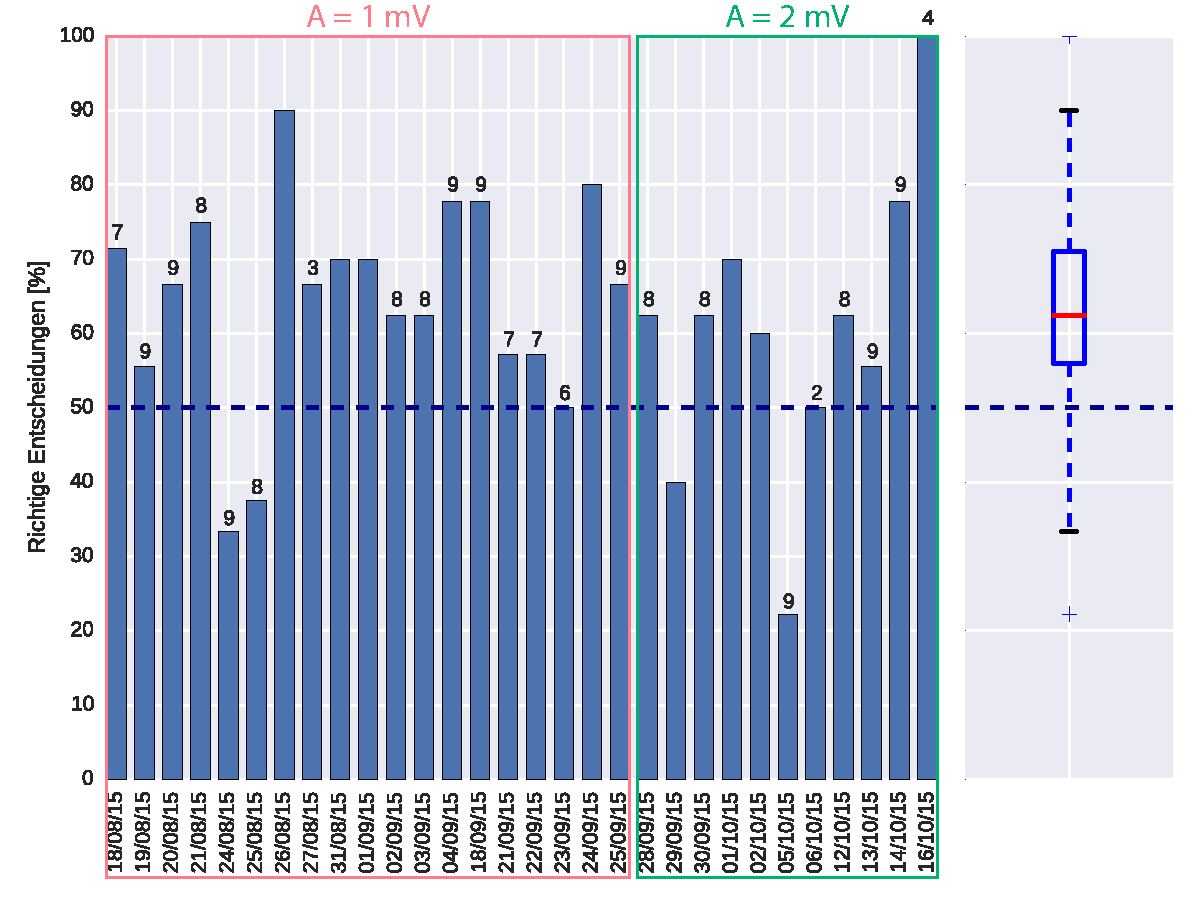
\includegraphics[height=8.5cm]{Abbildungen/Overview1}}
\subfigure[�bersicht Fisch 2]
{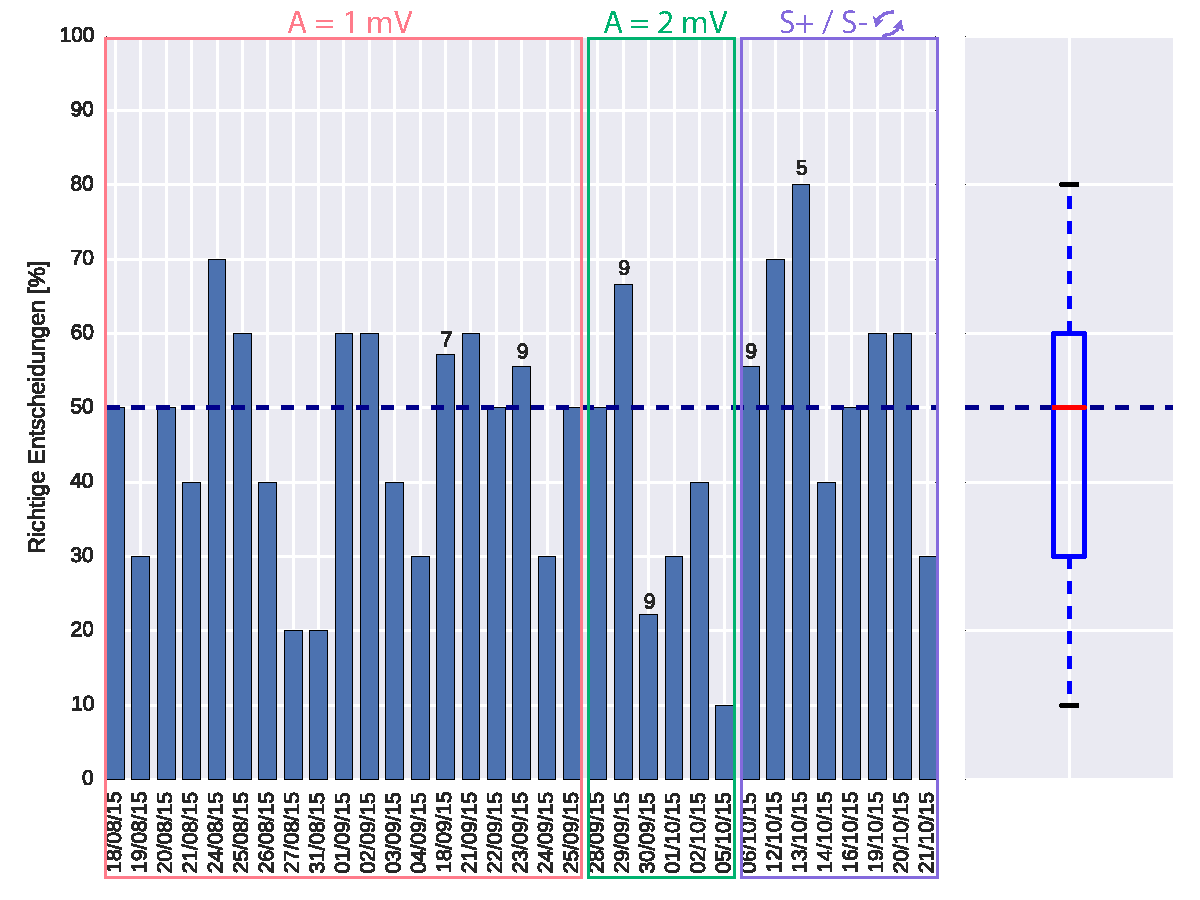
\includegraphics[height=8.5cm]{Abbildungen/Overview2}}
\caption{\label{fig:overview}�bersichtsabbildungen Hauptversuch f�r Fisch 1 (a) und Fisch 2 (b).  Links ist jeweils ein Balkendiagramm zu sehen. Dieses zeigt die Leistungen der Versuchstiere an allen Versuchstagen des Hauptversuchs in Prozent.  Die Zahlen �ber den einzelnen Balken, geben an, bei wie vielen der zehn Versuchsdurchl�ufen eine Entscheidung getroffen wurde. Steht keine Zahl �ber dem Balken, hat sich der Fisch bei allen zehn Versuchsdurchl�ufen entschieden. Rechts davon ist jeweils ein Boxplot, der die Verteilung der richtigen Entscheidungen �ber die gesamte Versuchszeit zeigt.}
\end{figure}

\subsection{Ver�nderung der Stimulusamplitude}

Im Folgenden werden die Leistungen der Versuchstiere bei einer Stimulusst�rke von einem Millivolt mit den Leistungen bei einer Stimulusst�rke von zwei Millivolt verglichen. Ziel des Vergleichs war es herauszufinden, ob die Stimulusamplitude einen Einfluss auf das Elektrodenauswahlverhalten der Tiere hat.
Die Versuchstiere wurden zun�chst bei einer Stimulusamplitude von einem Millivolt trainiert. Abbildung \ref{fig:amplitude1} (a) zeigt dabei die Leistungen von Fisch 1 in einem Balkendiagramm: An 17 von 20 Versuchstagen liegt diese �ber 50 Prozent. Dennoch ist kein kontinuierlicher Anstieg der Leistung mit ansteigender Zahl an absolvierten Versuchstagen zu erkennen, vielmehr schwanken Leistungen des Versuchstieres scheinbar willk�rlich. Im Median w�hlte Fisch 1 bei einer Stimulusamplitude von einem Millivolt in 66,7 Prozent der F�lle die richtige Elektrode aus. Der Binomialtest erbrachte f�r diese Verteilung einen P-Wert von 0,000116. Das Versuchstier hat sich also signifikant h�ufiger f�r die richtige Elektrode entschieden.  
Fisch 2 hingegen erbrachte beim Training mit einem Stimulus der Amplitude ein Millivolt, wie in Abbildung \ref{fig:amplitude1} (b) zu sehen, deutlich geringere Leistungen als Fisch 1. Seine Leistung lag lediglich an sieben der 20 Versuchstage �ber 50 Prozent. Der Median der Leistungsverteilung liegt dabei genau bei 50 Prozent.Der Binomialtest ergab dementsprechend einen recht hohen P-Wert von 0,2839. 

Da die Versuchstiere oftmals direkt eine der beiden zur Wahl stehenden Elektroden ausw�hlten, ohne sich vorher der anderen zu n�hern, wurde die Signalst�rke von einem Millivolt auf zwei Millivolt erh�ht, um die M�glichkeit die Signale aus einer gr��eren Entfernung wahrzunehmen zu erh�hen.
Wie in Abbildung \ref{fig:amplitude2} (a) zu sehen, nahm die Leistung von Fisch 1 am ersten Versuchstag nach der Umstellung der Stimulusamplitude zun�chst etwas ab, stieg dann aber wieder von 40 Prozent auf �ber 60 Prozent an. Jedoch ist auch hier kein kontinuietlicher Anstieg der Leistung �ber die Versuchstage hinweg zu beobachten. So kommt es ebenfalls zu pl�tzlichen Leistungseinbr�chen wie am f�nften Versuchstag nach der Umstellung auf 20 Prozent. Gegen Ende des Versuchs ist dann eine kontinuierlicher Anstieg der Leistung zu sehen. Dieser geht jedoch mit einem Anstieg der F�lle, in welchen der Fisch keine Entscheidung trifft einher. So hat sich Fisch 1 am letzten Versuchstag zwar in hundert Prozent der F�llen, in welchen er sich entschieden hat, richtig entschieden, allerdings hat er sich nur in vier von zehn Versuchsdurchl�ufen �berhaupt f�r eine Elektrode entschieden. Insgesamt lag Fisch 1 an sieben von zehn Versuchstagen in seinen Entscheidungen �ber der 50 Prozentgrenze. Hierbei ergibt sich eine mediane Leistung von 61,3 Prozent. Der P-Wert des Binomialtests von 0,1766 ist nicht signifikant. 
Vergleicht man nun die Leistungen von Fisch 1 bei einer Amplitude von einem Millivolt mit den Leistungen bei einer Amplitude von zwei Millivolt mit Hilfe eines unabh�ngigen t-Tests, so ergibt ein P-Wert von 0,489. Die Leistungen von Fisch 1 h�ngen also nicht wesentlich von der Amplitude ab.
Die Leistungen von Fisch 2 hingegen gingen nach der Umstellung auf eine Stimulusst�rke von zwei Millivolt stark zur�ck (siehe Abb. \ref{fig:amplitude2} b). Zwar stieg die Rate an Entscheidungen f�r die richtige Elektrode am ersten Tag der Umstellung kurzfristig auf 60 Prozent an, an den folgenden Versuchstage lag sie jedoch unter der 50 Prozentgrenze. Der Median der richtigen Entscheidungen lag somit bei 30 Prozent. Der P-Wert des Binomialtests betrug 0,029, was anzeigt, dass sich Fisch 1 signifikant h�ufiger f�r die falsche Elektrode als f�r die richtige Elektrode entschieden hat. Der t-Test zur �berpr�fung, ob sich die Leistungen von Fisch 2 bei den beiden verschiedenen Stimulusamplituden signifikant voneinander unterscheiden ergab hierbei einen P-Wert von 0,13.

\begin{figure}[H]
\subfigure[Fisch 1]
{\includegraphics[height=6cm]{Abbildungen/Performanceamplitude_is_one2015albi02}}
\subfigure[Fisch 2]
{\includegraphics[height=6cm]{Abbildungen/Performanceamplitude_is_one2015albi01}}
\caption{\label{fig:amplitude1} Balkendiagramm und Boxplot von Fisch 1 (a) und Fisch 2 (b) bei einer Stimulusamplitude von einem Millivolt.}
\end{figure}


\begin{figure}[H]
\subfigure[Fisch 1]
{\includegraphics[height=6cm]{Abbildungen/Performanceamplitude_is_two2015albi02}}
\subfigure[Fisch 2]
{\includegraphics[height=6cm]{Abbildungen/Performanceamplitude_is_two2015albi01}}
\caption{\label{fig:amplitude2} Balkendiagramm und Boxplot von Fisch 1 (a) und Fisch 2 (b) bei einer Stimulusamplitude von zwei Millivolt.}
\end{figure}


\subsection{S+ und S- Vertauscht}
Da sich Fisch 2 bei einer Stimuluselektrode von zwei Millivolt signifikant???? h�ufiger f�r die Elektrode entschied, welche den unbelohnten Stimulus abgab, sollte im Folgenden �berpr�ft werden, ob eine nat�rliche Pr�ferenz zum unbelohnten S- Stimulus besteht. Sollte dies der Fall sein, w�re ein deutlicher Leistungsanstieg von Fisch 2 aufgrund der zus�tzlichen positiven Verst�rkung zu erwarten.
Abbildung \ref{fig:getauscht} zeigt die Leistungen von Fisch 2, nachdem der S+ und der S- Stimulus vertauscht worden waren. Der neue S+ Stimulus war demnach ein eigenmanniaartiges Signal, w�hrend der neue S- Stimulus nun das rein sinusf�rmige Signal mit einem Frequenzunterschied zur Fisch EOD Frequenz von 60 Hertz war.
In den ersten drei Versuchstagen nach der Umstellung, ist ein kontinuierlicher Anstieg der Leistung auf bis zu 80 Prozent zu beobachten. Dies hatte Fisch 2 zuvor an noch keinem Versuchstag erreicht. An den folgenden Tagen sinkt die Leistung jedoch wieder auf unter 50 Prozent ab.
Insgesamt erreichte Fisch 2 an f�nf der acht Versuchstage einen Rate an richtigen Entscheidungen �ber 50 Prozent. Die mediane Leistung betrug 57,8 Prozent. Der Binomialtest ergab hierbei einen P-Wert von 0,561. Fisch 1 entschied sich also nicht signifikant h�ufiger f�r den belohnten Stimulus.

\begin{figure}[ht]
\centering
\includegraphics[height=8.5cm]{Abbildungen/performance_chap_changed_stimuli2015albi01}
\caption{\label{fig:getauscht}Die Leistungen von Fisch 2, nachdem der S+ und S- Stimulus vertauscht wurden. Links: Balkendiagramm, rechts: Boxplot.}
\end{figure}


\section{Hauptversuch - Videotrackingauswertung}
Jeder Versuchsdurchlauf des Hauptversuchs wurde auf Video aufgenommen. Dabei wurde das Video gestartet, bevor die Startbox ge�ffnet wurde. Beendet wurde das Video bevor die Belohnung stattfand oder der Fisch zur�ck in die Startbox gef�hrt wurde.
Die Videodateien wurden dann, wie bereits im Kapitel Datenanalyse erl�utert, mit Hilfe eines Trackingprogramms analysiert.

\subsection{Einzelvideoauswertung anhand eines Beispielvideos}

Im Folgenden wird zun�chst anhand der Auswertung eines einzelnen Beispielvideos erl�utert, wie die Auswertung aller Videos ablief und welche Parameter zur Bewertung eines Versuchsdurchlaufs wichtig sind.

\begin{figure}[ht]
\centering
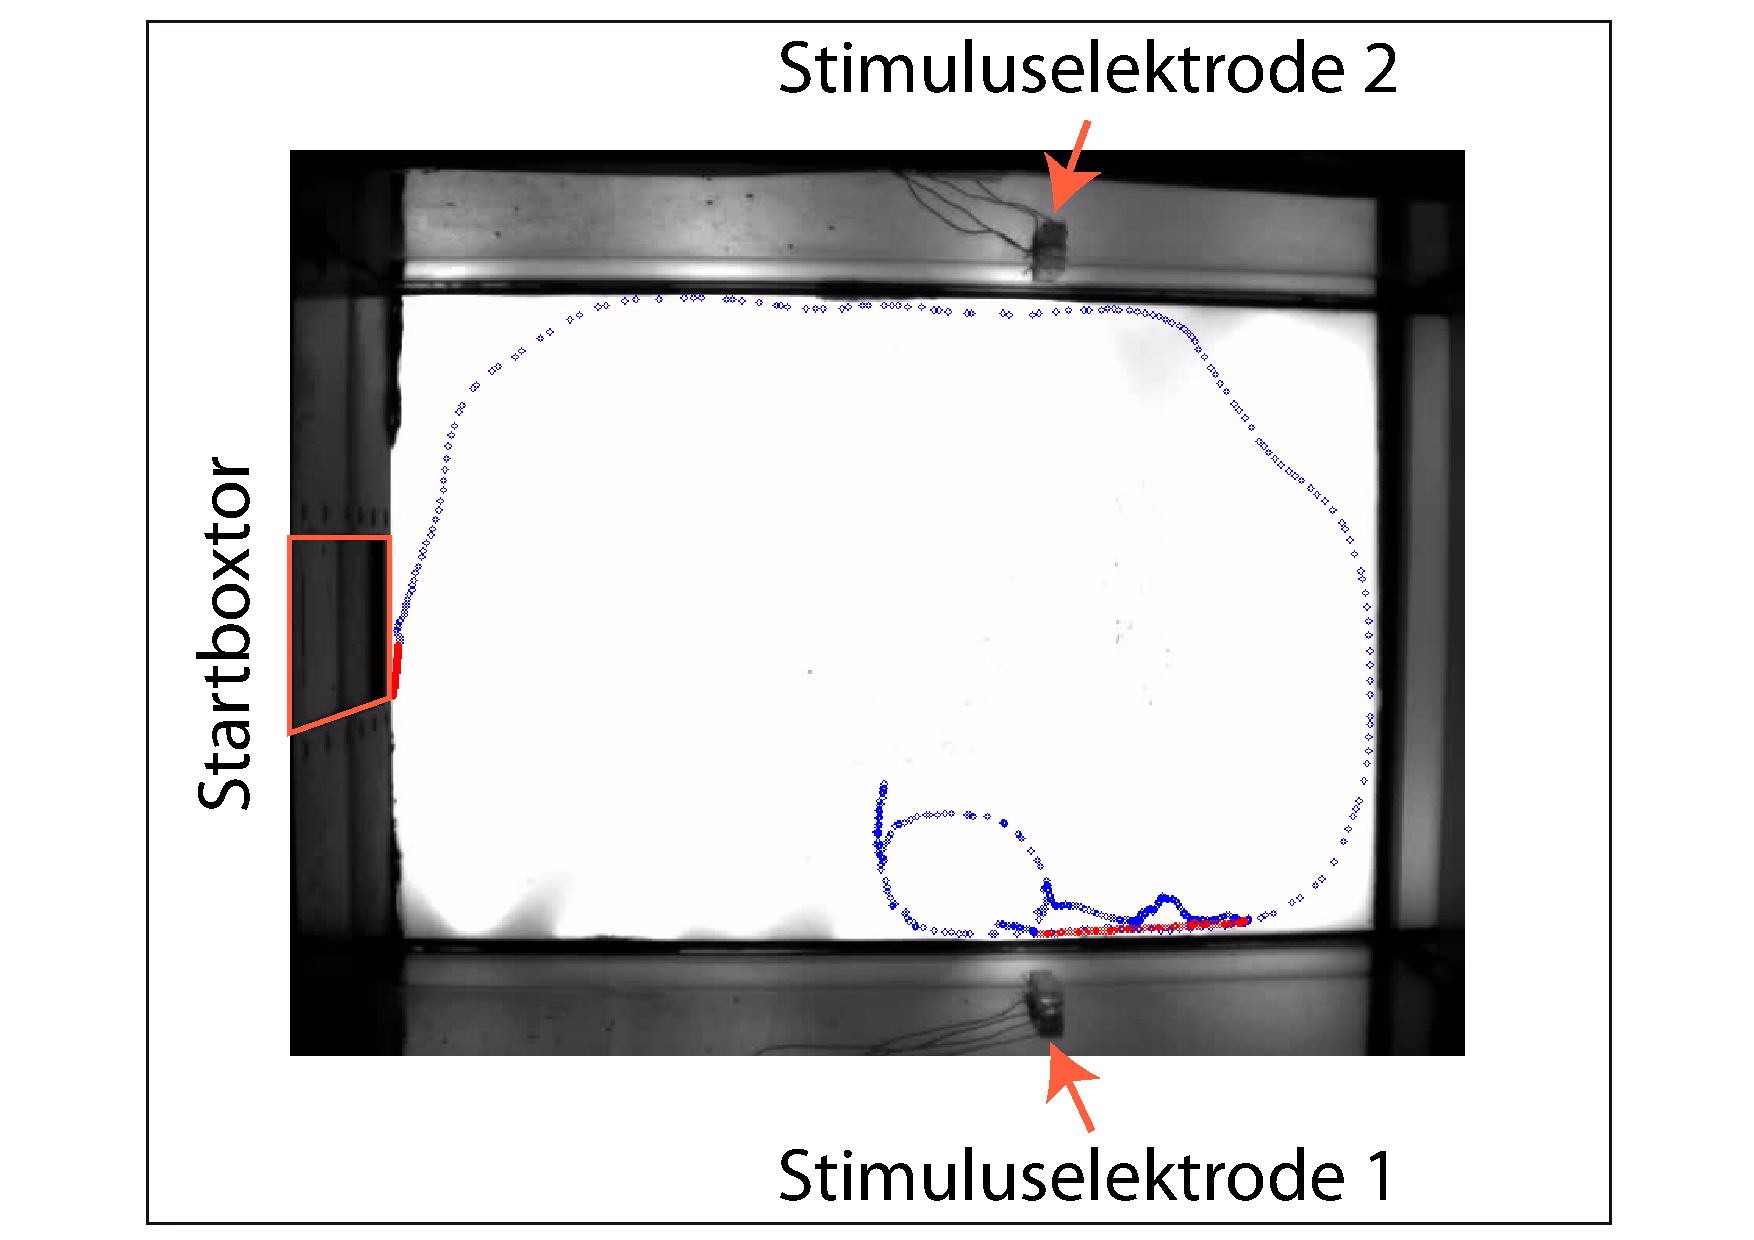
\includegraphics[height=8.5cm]{Abbildungen/2015-08-18_1_OV_path}
\caption{\label{fig:path} Ergebnissbild des Videotrackingprogramms. Das Trackingprogramm erstellt f�r jedes getrackte Video, ein Bild, welches den zur�ckgelegten Weg des Fisches zeigt. Die blauen Punkte sind Postitionen, an welchen sich das Versuchstier sicher befand. Die roten Punkte sind gesch�tzte Positionen, an welchen das Trackingprogramm den Fisch kurzzeitig verloren hatte.}
\end{figure}

Zun�chst wurde das Video mit dem Trackingprogramm getrackt, dabei wurden die X und Y Position im Versuchsbecken und die Orientierung des Versuchstiers f�r jedes Videoframe in jeweils einer Liste gespeichert. Au�erdem wurde eine Graphik erstellt, welche den w�hrend des Versuchsdurchlaufs zur�ckgelegten Weg des Fisches zeigt (siehe Abb. \ref{fig:path}).
In dem hier dargestellten Versuchsdurchlauf von Fisch 2 gab Elektrode 1 den belohnten Stimulus ab. Anhand des blauen Pfades in Abbildung \ref{fig:path} ist zu sehen, dass Fisch 2 zun�chst Elektrode 2 passierte und anschlie�end bei Elektrode 1 im Kreis geschwommen ist. Im Folgenden sollten Parameter gefunden werden, welche anzeigen, dass eine Elektrode ausgew�hlt wurde.

\begin{figure}
\subfigure[Elektrode 1]
{\includegraphics[height=5.5cm]{Abbildungen/distance_time_plot_2015-08-18_1_electrode1}}
\subfigure[Elektrode 2]
{\includegraphics[height=5.5cm]{Abbildungen/distance_time_plot_2015-08-18_1_electrode2}}
\caption{\label{fig:distanzen}Die Distanzen im Beispielversuchsdurchlauf von Fisch 2 zu Elektrode 1 (a) und Elektrode 2 (b)�ber die Zeit.}
\end{figure}

\begin{figure}[ht]
\centering
\includegraphics[height=8.5cm]{Abbildungen/Orientierung_2015-08-18_1}
\caption{\label{fig:orientierung}Orientierung}
\end{figure}

Um zu �berpr�fen, ob und wie nah sich das Versuchstier bei einem Versuchsdurchlauf an den Elektroden befand, wurden daher zun�chst die Distanzen des Versuchstiers zu jeder Elektrode zu jedem Zeitpunkt berechnet. Abbildung \ref{fig:distanzen} zeigt hierbei die f�r das Beispielvideo entstandenen Graphen, wobei in (a) die Distanz zu Elektrode 1 und in (b) die Distanz zu Elektrode 2 �ber die Zeit aufgetragen ist. Hierbei wird sichtbar, dass sich Fisch 2 im Beispiel auf lange Sicht Elektrode 1 ann�hert, w�hrend sich die Distanz zu Elektrode 2 nur kurz verringert.
Im weiteren wurden die Orientierung des Versuchstieres zu den Elektroden und die Schwimmgeschwindigkeit des Versuchstieres an den Elektroden untersucht. In Abbildung \ref{fig:orientierung} sind die Orientierungen des Fisches an den Elektroden mittles blauer Pfeile aufgetragen. Die L�nge der Pfeile kodiert dabei die Geschwindigkeit. Wie in der Abbildung zu sehen, schwamm Fisch 2 zun�chst im 90 Gradwinkel an Elektrode 2 vorbei und orientierte sich dann mehrfach zu Elektrode 1 hin. Desweiteren ist anhand der Pfeill�ngen zu beobachten, dass das Versuchstier kurz vorm Erreichen beider Elektroden seine Geschwindigkeit verringert. 

\subsection{Video�bergreifende Auswertung}

Im n�chsten Schritt sollten die in der Einzelvideoauswertung erlangten Erkenntnisse genutzt werden, um nun alle Videos eines Versuchstieres quantitativ auswerten zu k�nnen. Da wie in der Einzelvideoauswertung aufgezeigt die Distanz zu den Elektroden und die Schwimmgeschwindigkeit an den Elektroden wichtige Faktoren zu Bewertung der Auswahl einer Elektrode darstellen, wurden im weiteren diese beiden Faktoren betrachtet. Die Orientierung des Fisches eignet sich weniger zur Standardisierung, da diese sich h�ufig �ndert und kein deutliches Muster bei der Auswahl einer Elektrode erkennbar war.

Dabei wurden bei Fisch 1 insgesamt 274 Videos und bei Fisch 2 eine Anzahl von 324 Videos ausgewertet.
Die Datens�tze f�r Fisch 4 und Fisch 6 waren wegen geringer kooporation bei den Versuchen mit 42 Videos f�r Fisch 4 und 82 Videos f�r Fisch 6 wesentlich kleiner.

\begin{figure}[ht]
\subfigure[Fisch 1]
{\includegraphics[height=5.5cm]{Abbildungen/Histogramm_Elektrodendistanzen3_2015albi02}}
\subfigure[Fisch2]
{\includegraphics[height=5.5cm]{Abbildungen/Histogramm_Elektrodendistanzen3_2015albi01}}
\caption{\label{fig:histodistanzen}Histogramme Distanz zu den Elektroden}
\end{figure}

\begin{figure}[ht]
\subfigure[Fisch1]
{\includegraphics[height=5.5cm]{Abbildungen/roc_curve_E1Distanz22015albi02}}
\subfigure[Fisch 2]
{\includegraphics[height=5.5cm]{Abbildungen/roc_curve_E1Distanz22015albi01}}
\caption{\label{fig:roc_distanzen}Roc Kurven Distanzen}
\end{figure}

Da es wie aus den FuK Werten der ROC Kurven ersichtlich offenbar keine gro�e Rolle spielt, ob Elektrode 1 oder Elektrode 2 gew�hlt wurde, wurde im Folgenden Histogramme erstellt, welche unabh�ngig davon, welche Elektrode es war, zeigen wie die Distanzverteilung des Versuchstieres war, wenn die richtige Elektrode ausgew�hlt wurde und die Distanz zur richtigen Elektrode wenn die falsche Elektrode ausgew�hlt wurde. Das Ergebnis f�r Fisch 1 ist dabei in Abbildung \ref{fig:histodistanzen} (a) zu sehen. Abbildung \ref{fig:histodistanzen} (b) zeigt das gleiche f�r Fisch 2. Wie zu erwarten, Hielten sich die Versuchstiere h�ufiger nah an der richtigen Elektrode auf, wenn diese ausgew�hlt wurde. Dementsprechend waren die Distanzen zur richtigen Elektrode h�her, wenn die falsche Elektrode ausgew�hlt wurde.
Die ROC Kurven der Histogramme haben dementsprechend auch eine FuK �ber 0,5 (siehe Abb. \ref{fig:roc_distanzen} (a) f�r Fisch 1 und Abb. \ref{fig:roc_distanzen} (b) f�r Fisch 2. Die FuK bei Fisch 1 betr�gt 0,63 w�hrend die von Fisch 2 0,73 betr�gt.

Zun�chst sollte untersucht werden, welche Distanzen zu einer Elektrode bestehen, wenn sie ausgew�hlt wurde. Hierf�r wurde um die beiden Elektroden ein Radius von 35 cm gelegt. Die daraus entstandenen Histogramme sind f�r Fisch 1 in Abbildung \ref{fig:histodistanzen_entscheidung1} zu sehen. Hierbei wurden f�r Elektrode 1 und Elektrode 2 je die richtig Positiven und die falsch Positiven aufgetragen. Unter E1 richtig positive versteht man die Distanzen zu Elektrode 1, wenn diese richtig war und vom Fisch ausgew�hlt wurde. Bei den E 1 falsch Positiven hingegen wurden die Distanzen zu Elektrode 1 aufgetragen, wenn Elektrode 1 falsch war aber dennoch vom Fisch gew�hlt wurde. Analog dazu wurden bei E2 richtig Positive und E2 falsch Postive die Distanzen zu Elektrode 2 aufgetragen.
Fisch 1 hat dabei insgesamt eine starke Anh�ufung von kurzen Distanzen, bei den E1 falsch Positiven. Das hei�t er hat sich h�ufig nah an Elektrode 1 aufgehalten, wenn diese falsch war und er sie au�gew�hlt hat.

DISKUSSION: M�gliche Gr�nde daf�r: m�glicherweise observer bias, sprich wenn fisch noch nicht so nah an elektrode war, wurde das fr�her als richtige entscheidung gez�hlt und wenn fisch an der falschen elektrode war wurde l�nger gewartet. m�glicherweise liegt der grund auch im ablauf: wenn der fisch die falsche elektrode ausgew�hlt hat, bekam er direkt ein feedback da der stimulus gleich aus ging. wenn der fisch richtig gew�hlt hat wurde das video ausgeschaltet, aber der stimulus angelassen und der fisch musste noch einige zeit an elektrode verweilen und auf die belohnung warten, was aber vom video nicht erfasst wurde. wenn der fisch in dieser zeit wieder weggeschwommen ist, wurde der versuch auch nicht als richtig gewertet.


\begin{figure}[ht]
\centering
\includegraphics[height=8.5cm]{Abbildungen/Histogramm_Elektrodendistanzen_mit_Fischentscheidung2015albi02}
\caption{\label{fig:histodistanzen_entscheidung1}Fisch 1 Histogramme zur Distanz zu den Elektroden mit fischentscheidung}
\end{figure}

\begin{figure}[ht]
\subfigure[Roc Kurve Elektrode 1]
{\includegraphics[height=5.5cm]{Abbildungen/roc_curve_E1Distanz2015albi02}}
\subfigure[Roc Kurve Elektrode 2]
{\includegraphics[height=5.5cm]{Abbildungen/roc_curve_E2Distanz2015albi02}}
\caption{\label{fig:roc_distanzen_entscheidung1}Roc Kurven dazu von Fisch 1}
\end{figure}


Um zu �berpr�fen, ob es Unterschiede in den Verteilungen gibt, wenn es richtig Positiv ist und falsch Postitiv ist. Sprich um zu �berpr�fen, ob die Distanzen zu den Elektroden unterschiedlich verteilt waren, je nach dem ob die Elektrode, die der Fisch ausgew�hlt hat, richtig oder falsch war, wurden ROC Kurven erstellt.
Diese sind in Abbildung \ref{fig:roc_distanzen_entscheidung1} zu sehen. Es wurde jeweils eine Kurve f�r Elektrode 1 (siehe Abb \ref{fig:roc_distanzen_entscheidung1} (a)) und eine f�r Elektrode 2 (siehe Abb. \ref{fig:roc_distanzen_entscheidung1} (b) ertellt. Auf der X-Achse ist jeweils die Falsch Positiv Rate dargestellt, w�hrend auf der Y-Achse die richtig Positiv Rate aufgetragen ist. Die Abk�rzung FuK steht f�r "Fl�che unter der Kurve". Der Wert gibt also wie der Name bereits verr�t die Fl�che unter der ROC Kurve an. L�ge der Wert bei 0,5 dann w�ren beide Verteilungen gleich??? Je kleiner der Wert ist desto mehr sind die Werte zum Falsch Positiven hin verschoben, je gr��er die Fl�che ist, desto mehr sind die Werte zum richtig positiven verschoben.

Mit der gleichen Vorgehensweise wurde anschlie�end bei Fisch 2 gearbeitet. Das so entstandene Histogramm ist in Abbildung \ref{fig:histodistanzen_entscheidung2} zu sehen. �hnlich wie bei Fisch 1 kommen auch hier bei den falsch Positiv Kategorien f�r Elektrode 1 und Elektrode 2 h�ufiger kurze Distanzen vor, als bei den richtig Positiv Kategorien.
%\begin{figure}[ht]
%\includegraphics[height=10.5cm]{Abbildungen/Histogramm_Elektrodendistanzen_mit_Fischentscheidung2015albi01}
%\caption{\label{fig:histodistanzen_entscheidung2}Fisch 2 Histogramme zur Distanz zu den Elektroden mit fischentscheidung}
%\end{figure}

Auch die ROC Kurven von Fisch 2 (siehe Abb. \ref{fig:roc_distanzen_entscheidung2} sind vergleichbar mit den Kurven von Fisch 1. So betr�gt die FuK von Elektrode 1 0,35 (bei Fisch 1 waren es 0,37) und bei Elektrode 2 0,41 (bei Fisch 1: 0,42).


%\begin{figure}[ht]
%\subfigure[Roc Kurve Elektrode 1]
%{\includegraphics[height=6cm]{Abbildungen/roc_curve_E1Distanz2015albi01}}
%\subfigure[Roc Kurve Elektrode 2]
%{\includegraphics[height=6cm]{Abbildungen/roc_curve_E2Distanz2015albi01}}
%\caption{\label{fig:roc_distanzen_entscheidung2}Roc Kurven dazu von Fisch 2}
%\end{figure}


Ein weiterer Faktor, welcher zur Bewertung, ob die Fische eine Elektrode ausgew�hlt haben herbeigezogen wurde, war die Schwimmgeschwindigkeit. Daf�r wurden zun�chst die Geschwindigkeiten nahe der Elektroden mit den Geschwindigkeiten entfernt von den Elektroden verglichen. Als nahe den Elektroden wurde eine Distanz zu den Elektroden von maximal 12 Zentimetern festgelegt. Jede gr��ere Distanz und die dazu geh�rige Geschwindigkeit wurde zu entfernt von den Elektroden gez�hlt. Abbildung \ref{fig: boxplot_geschwindigkeit} (a) zeigt in Form eines Boxplots die Verteilung der Schwimmgeschwindigkeiten von Fisch 1 in der N�he und entfernt von den Elektroden. Die mediane Schwimmgeschwindigkeit in der N�he der Elektroden betrug dabei 6,34 Zentimeter pro Sekunde. Der Median der entfernten Geschwindigkeit hingegen lag bei 8,21.
Ein Mann-Whitney U test Test ergab hierbei einen P-Wert von 0. Bei einer Datenmenge von 118538 Werten.
F�r Fisch 2 zeigt sich �hnliches: Wie in Abbildung \ref{fig: boxplot_geschwindigkeit} (b) zu sehen, war die Schwimmgeschwindigkeit von Fisch 2 ebenfalls in der N�he der Elektroden niedriger. So ergab sich hier ein Median von 3,44 Zentimeter pro Sekunde in der N�he der Elektroden, w�hrend die mediane Geschwindigkeit entfernt von den Elektroden 6,01 Zentimeter pro Sekunde betrug. Der Mann-Whitney U test Test ergab hier ebenfalls einen P-Wert von 0 bei einer Datenmenge von 89265 Werten.


\begin{figure}[ht]
\subfigure [Fisch 1]
{\includegraphics[height=5.5cm]{Abbildungen/Velocityboxplot2015albi02}}
\subfigure[Fisch 2]
{\includegraphics[height=5.5cm]{Abbildungen/Velocityboxplot2015albi01}}
\subfigure[Fisch 4]
{\includegraphics[height=5.5cm]{Abbildungen/Velocityboxplot2013albi14}}
\subfigure[Fisch 6]
{\includegraphics[height=5.5cm]{Abbildungen/Velocityboxplot2012albi01}}
\caption{\label{fig: boxplot_geschwindigkeit} Geschwindigkeits Boxplots}
\end{figure}

Bei Fisch 4 (siehe Abb. \ref{fig: boxplot_geschwindigkeit} (c) und Fisch 6 (siehe Abb. \ref{fig: boxplot_geschwindigkeit} (d) hingegen zeigt sich eine umgekehrte Tendenz: Hier sind die Fische an den Elektroden sogar etwas schnelle (Median in der N�he der Elektroden: Fisch 4: 11,8 Zentimeter pro Sekunde, Fisch 6: 9,81 Zentimeter pro Sekunde.

Median entfernt von den Elektroden: Fisch 4: 9,15 Zentimeter pro Sekunde, Fisch 6: 9,03 Zentimeter pro Sekunde. Grund hierf�r ist vermutlich, dass die Fische im Gegensatz zu Fisch 1 und 2 die Aufgabe nicht verstanden haben. Da die Elektroden an den an den Beckenl�ngsseiten angebracht ist, schwimmen die Fische dort vermutlich schnell vorbei.
Mann-Whitney U test Test: P-Wert Fisch 4: 4,85 x 10 hoch -20, datenmenge von 35176
Mann-Whitney U test Test: P-Wert Fisch 6: 0,00073, datenmenge von 50465

F�r Fisch 1 und Fisch 2 wurden dann nochmal die Geschwindigkeiten an ELektrode 1 und 2 verglichen, wenn die Elektrode richtig und ausgew�hlt war mit dem Fall, dass die Elektrode Falsch und ausgew�hlt war. Abbildung \ref{fig: histo_geschwindigkeit1} zeigt dazu die Histogramme f�r Fisch 1. Wie in der Abbbildung zu sehen, unterscheiden sich die Histogramme nicht wesentlich voneinander. Auch die ROC Kurven f�r Elektrode 1 (siehe Abb. \ref{fig:roc_geschwindigkeiten_entscheidung1}) und f�r Elektrode 2 \ref{fig:roc_geschwindigkeiten_entscheidung2} fallen dementsprechend aus: Mit einer FuK von 0,45 bzw. 0,44 zeigen beide ROC Kurven, dass sich die Histogramme nicht wesentlich voneinander unterscheiden, egal ob der Fisch die richtige oder die Falsche Elektrode ausgew�hlt hat.

\begin{figure}[ht]
\centering
\includegraphics[height=8.5cm]{Abbildungen/Histogramm_Geschwindigkeiten_mit_Fischentscheidung2015albi02}
\caption{\label{fig: histo_geschwindigkeit1} Fisch 1}
\end{figure}

\begin{figure}[ht]
\subfigure[Roc Kurve Elektrode 1]
{\includegraphics[height=5.5cm]{Abbildungen/roc_curve_E1Geschwindigkeit2015albi02}}
\subfigure[Roc Kurve Elektrode 2]
{\includegraphics[height=5.5cm]{Abbildungen/roc_curve_E2Geschwindigkeit2015albi02}}
\caption{\label{fig:roc_geschwindigkeiten_entscheidung1}Roc Kurven Geschwindigkeiten mit Entscheidung von Fisch 1}
\end{figure}

Analog dazu wurden auch f�r Fisch 2 die entsprechenden Histogramme erstellt, wie in Abbildung \ref{fig: histo_geschwindigkeit2} zu sehen. Hier unterscheiden sich die Histogramme auf den ersten Blick etwas st�rker, so ist das Peak bei E1 falsch und ausgew�hlt etwas h�her als bei E1 richtig und ausgew�hlt.
Die ROC Kurven (siehe Abb. \ref{fig:roc_geschwindigkeiten_entscheidung2}) aber zeigen, dass auch hier kein nennenswerter Unterschied besteht. So betr�gt die FuK bei Elektrode 1 0,41 und bei Elektrode 2 0,45.


%\begin{figure}[ht]
%\includegraphics[height=10.5cm]{Abbildungen/Histogramm_Geschwindigkeiten_mit_Fischentscheidung2015albi01}
%\caption{\label{fig: histo_geschwindigkeit2} Fisch 2}
%\end{figure}

%\begin{figure}[ht]
%\subfigure[Roc Kurve Elektrode 1]
%{\includegraphics[height=6cm]{Abbildungen/roc_curve_E1Geschwindigkeit2015albi01}}
%\subfigure[Roc Kurve Elektrode 2]
%{\includegraphics[height=6cm]{Abbildungen/roc_curve_E2Geschwindigkeit2015albi01}}
%\caption{\label{fig:roc_geschwindigkeiten_entscheidung2}Roc Kurven Geschwindigkeiten mit Entscheidung von Fisch 1}
%\end{figure}


\begin{figure}[ht]
\subfigure[Fisch 1]
{\includegraphics[height=6.5cm]{Abbildungen/Heatmap_positions2015albi02}}
\subfigure[Fisch 2]
{\includegraphics[height=6.5cm]{Abbildungen/Heatmap_positions2015albi01}}
\subfigure[Fisch 4]
{\includegraphics[height=6.5cm]{Abbildungen/Heatmap_positions2013albi14}}
\subfigure[Fisch 5]
{\includegraphics[height=6.5cm]{Abbildungen/Heatmap_positions2013albi09}}
\subfigure[Fisch 6]
{\includegraphics[height=6.5cm]{Abbildungen/Heatmap_positions2012albi01}}
\caption{\label{fig: heatmap_positions} Positionen im Becken, an denen sich die Fische w�hrend der Versuche h�ufig aufgehalten haben. Der rote Punkt stellt Elektrode 1 dar, der blaue Punkt Elektrode 2.}
\end{figure}







%\chapter{Diskussion}

\section{Lernerfolg der Versuchstiere}
Bereits bei den Vorversuchen zeigte sich, dass Fisch 1 und Fisch 2 einen gr��eren Lernerfolg aufwiesen als Fisch 3 und Fisch 4. Bei dem ersten Vorversuch, der \emph{Eingew�hnung}, beispielsweise verringerten Fisch 1 und Fisch 2 die mittlere Zeit, die sie brauchten, um die Larve an den Elektroden zu finden, mit der Anzahl bereits absolvierter Versuchstage (siehe Abb. \ref{fig: versuch1_zeit}). Demnach lernten sie, dass an den Elektroden Futter zu finden war. Bei Fisch 3 und Fisch 4 hingegen schwankten die mittleren Zeiten stark. Bei beiden Tieren verl�uft die Zeitkurve in einem zickzackartigen Muster. Besonders bei Fisch 4 f�llt auf, dass auf einen erfolgreichen Versuchstag, an dem das Versuchstiere viele Larven fand und verzehrte, ein schwacher Tag mit schlechter Kooperation folgte. Man k�nnte dieses Verhalten m�glicherweise damit erkl�ren, dass die Versuchstiere nach einem erfolgreichen Versuchstag am n�chsten Tag keinen Hunger mehr hatten. Dagegen spricht jedoch, dass es sich bei den Tagen, an denen die Fische schlecht abschnitten, h�ufig um Montage handelte und zu erwarten gewesen w�re, dass die Tiere nach dem Wochenende hungrig sind. Au�erdem handelte es sich bei den unstet abschneidenden Versuchstieren (Fisch 3 und 4) um die ausgewachsenen Tiere, die etwa die doppelte K�rperl�nge der juvenilen (Fisch 1 und 2) ma�en, weshalb es unwahrscheinlich erscheint, dass letztere Hunger hatten, erstere aber nicht. 
Eine wahrscheinlichere Erkl�rung f�r das schnellere Lernen und das bessere Abschneiden der Jungtiere ist, dass die Versuche wenige Tage nach ihrer Lieferung gestartet wurden und sie an noch keinen F�tterungsablauf in der neuen Umgebung gew�hnt und daher lernf�higer als die adulten Tiere waren, die bereits seit einem (Fisch 3) oder sogar zwei (Fisch 4) Jahren nach einem festen F�tterungsablauf in ihrem Tank gef�ttert worden waren.
Was sich bereits im ersten Vorversuch gezeigt hatte, zog sich durch die weiteren Vorversuche und den Hauptversuch durch. So schnitten, wie in Abbildung \ref{fig: erfolgsquote} zu sehen, Fisch 1 und Fisch 2 auch bei den beiden weiteren Vorversuchen besser ab und konnten wegen geringerer Zeiten insgesamt mehr Versuchsdurchl�ufe pro Vorversuch absolvieren. Fisch 3 verweigerte die Teilnahme am letzten Vorversuch, indem er er die Startbox nicht freiwillig verlie�. Daher wurde das Versuchstier nicht zum Hauptversuch zugelassen.

Im Hauptversuch wurden zwei weitere Versuchstiere (Fisch 5 und 6) dazugenommen, die den Versuch schon im Rahmen einer vorangegangenen Bachelorarbeit neun Monate zuvor erlernt hatten. Als S+ und S- Stimulus wurden dieselben Beatfrequenzen wie damals gew�hlt. Beide Versuchstiere konnten sich aber anscheinend nicht mehr an den Versuchsablauf erinnern: Fisch 5 verlie� kaum einmal die Startbox; Fisch 6 kooperierte zwar besser und erkundete das Versuchsbecken, w�hlte aber keine Elektrode aus.  Die Versuchstiere erinnerten sich auch nach mehreren Durchl�ufen an verschiedenen Tagen nicht, was vermutlich daran lag, dass der versuchsfreie Zeitraum von neun Monaten zu lang war. Zumindest konnte bei der verwandten Art \emph{Apteronotus leptorhynchus} gezeigt werden, dass diese sich an die Beatfrequenzen ihrer Artgenossen nur einige Tage lang erinnern konnten \citep{Harvey-Girard2010}. M�glicherweise verf�gt \emph{Apteronotus albifrons} �ber eine �hnliche Erinnerungsspanne.

Beim Betrachten der Schwimmgeschwindigkeiten zeigte sich, dass Fisch 1 und Fisch 2 nahe der Elektroden signifikant langsamer schwammen als in gr��erer Entfernung (siehe Abb. \ref{fig: boxplot_geschwindigkeit}). Sie bremsten also ab, um eine Elektrode zu untersuchen und auszuw�hlen. Fisch 4 und Fisch 6 hingegen hatten im Bereich der Elektroden sogar sigifikant h�here Geschwindigkeiten als abseits von ihnen. Anscheinend hatten sie nicht erlernt, dass sie eine der beiden Elektroden ausw�hlen sollten, sondern schwammen an diesen vorbei. Dass sie an den Elektroden sogar deutlich h�here Geschwindigkeiten hatten, k�nnte m�glicherweise an der Elektroden-Position an den Beckenl�ngsseiten, sprich einer langen gerade Schwimmstrecke, liegen. Die Orte, die die Fische im Versuchsbecken h�ufig frequentierten (siehe Abb. \ref{fig: heatmap_positions}) zeigen ebenfalls, dass sich Fisch 1 und Fisch 2 deutlich h�ufiger an den Elektroden aufhielten als die �brigen Versuchstiere. Letztere hielten sich bevorzugt an den Beckenr�ndern auf, zeigten aber keine besondere Pr�ferenz f�r die Elektroden. Die Tiere meiden demnach offene Fl�chen.
 
In Konditionierungsversuchen zeigte \citet{Emde2007}, dass schwach elektrische Fische erlernen k�nnen, Objekte anhand ihrer Gr��e, Form oder ihres Materials zu unterscheiden und auszuw�hlen. Dar�ber konditionierte \citet{Knudsen1974} \emph{Apteronotus albifrons} darauf, eine Stimuluselektrode, die Sinusschwingungen verschiedener Frequenzen abgab, von einer solchen, die kein Signal aussendete, zu diskriminieren. Erwartungsgem�� sollte es \emph{Apteronotus albifrons} demnach m�glich sein, den in dieser Arbeit geforderten Versuchsablauf zu erlernen. Dennoch war die Aufgabe, eine Stimuluselektrode auszuw�hlen, f�r die Versuchstiere anscheinend komplex und schwierig. So erlernten lediglich zwei von vier Versuchstieren den Ablauf. Auch die beiden Versuchstiere Fisch 5 und 6, die erst beim Hauptversuch hinzugezogen wurden, den Versuch aber zuvor schon einmal erlernt hatten, waren nicht dazu in der Lage, die Aufgabe innerhalb der Hauptversuchszeit erneut zu erlernen.

\section{Einfluss abiotischer Faktoren}

Da es den Versuchstieren schwer viel, die Aufgabe zu erlernen, soll im Folgenden er�rtert werden, welche Faktoren den Lernerfolg beeintr�chtigt haben k�nnten.

\begin{figure}[ht]
\centering
\includegraphics[height=8.5cm]{Abbildungen/eod_boxplot}
\caption{\label{fig:eods}Die Verteilung der EOD-Frequenzen der Versuchstiere �ber den gesamten Versuchszeitraum gemessen. Die EOD-Frequenz von Fisch 1 betrug im Median 955 Hz bei einem Quartilsabstand (IQR) von 15 Hz. Die EOD-Frequenz von Fisch 2 lag etwas tiefer und betrug im Median 873 Hz bei einem IQR von 71 Hz. Fisch 3 hatte von allen Versuchstieren die h�chste EOD-Frequenz und lag bei einem Median von 1261 Hz. Hier betrug der IQR 24,5 Hz. Der Median von Fisch 4 befand sich bei 927 Hz mit einem IQR von 12 Hz. 907 Hz betrug die mediane EOD-Frequenz von Fisch 5 bei einem IQR von 9 Hz. Fisch 6 besa� mit einem Median von 1064.5 Hz die zweit h�chste EOD-Frequenz bei einem IQR von 34,25 Hz.}
\end{figure}

Wie Abbildung \ref{fig:eods} in einem Boxplot zu sehen ist, variierten die EOD-Frequenzen der Versuchstiere im Laufe des Versuchszeitraums. Die Boxl�nge entspricht dabei dem Quartilsabstand (IQR) und gibt an, wie weit die Daten gestreut sind. Die Schwankungen der EOD-Frequenzen sind vermutlich durch �nderungen der Wassertemperatur im Versuchsbecken zu erkl�ren. Dieser Zusammenhang wurde beispielsweise bereits von \citet{Enger1968} und \citet{Dunlap2000} beschrieben.

\begin{figure}[H]
\centering
\subfigure[Fisch1]
{\includegraphics[height=5.5cm]{Abbildungen/temperatur1}}
\subfigure[Fisch2]
{\includegraphics[height=5.5cm]{Abbildungen/temperatur2}}
\caption{\label{fig:temperatureod}Korrelation der Wassertemperaturen und EOD-Frequenzen. Links: Die Wassertemperaturen (rote Kurve) und die EOD-Frequenzen (gr�ne Kurve) von Fisch 1 (a) und Fisch 2 (b) �ber den gesamten Versuchszeitraum einschlie�lich der Vorversuche. Rechts:  Streudiagramm der EOD-Frequenzen und der zugeh�rigen Wassertemperatur aller Versuchsdurchl�ufe. In rot ist die daraus resultierende Regressionsgerade eingezeichnet.}
\end{figure}

F�r Fisch 1 konnte tats�chlich ein solcher Zusammenhang zwischen Wassertemperatur und der EOD-Frequenz gezeigt werden, wie in Abbildung \ref{fig:temperatureod} a) sichtbar wird. Der linke Graph zeigt die mittlere EOD-Frequenz (gr�ne Kurve) und die mittlere Wassertemperatur (rote Kurve) f�r jeden Versuchstag. �ber den gesamten Versuchszeitraum ist das Muster zu erkennen, dass Wassertemperatur und EOD-Frequenz gleicherma�en abfallen und ansteigen; beispielsweise sinken beide an Versuchstag f�nf stark ab. Rechts neben dem Graph ist ein zweiter mit einer Regressionsgeraden zu sehen. Hier wurden die EOD-Frequenzen und Wassertemperaturen jedes Versuchsdurchlaufs als Streudiagramm aufgetragen und die zugeh�rige Regressionsgerade berechnet. F�r Fisch 1 ergab sich hierbei ein Pearsons-Korrelationskoeffizient von 0,374 bei einem P-Wert von $1,6*10^{-15}$. Es liegt also anscheinend eine linearer Zusammenhang von Temperatur und EOD-Frequenz vor. Allerdings geben \citet{Dunlap2000} f�r die nahe verwandte Art \emph{Apteronotus leptorynchus} $r^2$-Werte von �ber 0,97 an. Es w�re also aufgrund der nahen Verwandtschaft auch f�r \emph{Apteronotus albifrons} eine st�rkere Korrelation von EOD-Frequenz und Wassertemperatur zu erwarten gewesen. Die Daten sind auff�llig weit gestreut. So wurden beispielsweise f�r Fisch 1 bei der Wassertemperatur $27,2^\circ$C EOD-Frequenzen zwischen 860 und 1000 Hertz gemessen. Erkl�ren l�sst sich das m�glicherweise dadurch, dass einzelne EOD-Frequenzen falsch gemessen wurden, da die Ableitung der Signale trotz Erdung durch andere elektrische Ger�te wie die Infrarotstrahler teilweise gest�rt wurde. Au�erdem ma� das verwendete Thermometer nur auf eine Dezimalstelle genau und brauchte recht lang um eine Temperatur�nderung zu registrieren, so dass die Wassertemperatur m�glicherweise nicht exakt genug ermittelt werden konnte. 

Die Daten von Fisch 2 zur Korrelation von Wassertemperatur und EOD-Frequenz (siehe Abb. \ref{fig:temperatureod} b) hingegen widersprechen den Erwartungen g�nzlich. Die EOD-Frequenz des Versuchstiers scheint im Laufe der Versuchstage abzunehmen, w�hrend die Wassertemperatur ansteigt. Die Regression ergibt entsprechend einen negativen Pearsons-Korrelationskoeffizienten von -0,314 bei einem P-Wert von $2,08*10^{-12}$. Da eine lineare Korrelation von EOD-Frequenzen und Wassertemperaturen bekannt ist \citep{Enger1968, Hopkins1976, Dunlap2000}, weichen diese Ergebnisse stark von den Erwartungen ab. Zus�tzlich weist Fisch 2 mit einem Quartilsabstand von 71 Hz eine weite Verteilung der EOD-Frequenzen auf (siehe Abb. \ref{fig:eods}). Aufgrund der starken Schwankungen der EOD-Frequenz von Fisch 2 und der nicht vorhandenen positiven Korrelation mit der Wassertemperatur, k�nnte ein Messfehler beim Erfassen der EOD-Frequenzen von Fisch 2 vorliegen. Allerdings erscheint dies unwahrscheinlich, da die EOD-Messung bei den anderen Versuchstieren funktionierte. Weshalb die EOD-Frequenzen von Fisch 2 sich antiproportional zur Wassertemperatur verhielten, bleibt daher zun�chst ungekl�rt.

\begin{table}[ht] 
	\centering
	\caption{ Mediane $Q_{10}$-Werte aller Versuchstiere. Die Werte wurden wie folgt berechnet: Zun�chst wurde f�r jeden Versuchstag und jedes Versuchstier ein $Q_{10}$-Wert aus der maximalen (T2) und minimalen (T1) Wassertemperatur des Versuchstages und den dazugeh�rigen EODs (E1, E2) mit folgender Formel berechnet $Q_{10} = \frac{E2}{E1}^{ \frac{10}{T2-T1}}$. Anschlie�end wurde der Median aus den $Q_{10}$-Werten aller Versuchstage berechnet.}
	\vspace{0,2cm}	
	\begin{tabular}{cccc} %eigentliche Tabelle 
		\toprule % d�nne Linie 
			& $Q_{10}$-Wert \\
		 Fisch 1 (2015albi02):& 1,31 \\
		 Fisch 2 (2015albi01):& 1,33 \\
		 Fisch 3 (2014albi08):& 1,23 \\
		 Fisch 4 (2013albi14):& 1,37 \\
		 Fisch 5 (2013albi09):& 1,25 \\
		 Fisch 6 (2012albi01):& 1,37 \\
		\bottomrule % bi�chen dickere Linie unten
	\end{tabular}
	\label{q10}
\end{table}


Um zu �berpr�fen, ob die Anpassungen der EOD-Frequenzen der Versuchstiere an die Wassertemperatur generell im Normalbereich lagen, wurde zus�tzlich der so genannte $Q_{10}$-Wert bestimmt, ein g�ngiges Ma� f�r diesen Zusammenhang. Er gibt an, um welchen Faktor die EOD-Frequenz des Versuchstieres bei einer Erw�rmung der Wassertemperatur um 10 Kelvin ansteigt (siehe Tabelle \ref{q10}). Hierbei ergab sich f�r alle Versuchstiere im Mittel ein $Q_{10}$-Wert von 1,3. In der Literatur werden f�r die Gattung \emph{Apteronotus} $Q_{10}$-Werte im Bereich von 1,5 \citep{Hopkins1976} bis 1,6 \citep{Dunlap2000} angegeben. Grund f�r den niedrigeren $Q_{10}$-Wert in diesem Experiment k�nnte die eingeschr�nkte Messgenauigkeit des verwendeten Thermometers gewesen sein, welches lediglich eine Nachkommastelle angab.


\begin{figure}[ht]
\centering
\includegraphics[height=7.5cm]{Abbildungen/conductivity}
\caption{\label{fig:conductivity}Korrelation von Leitf�higkeit und EOD-Frequenz bei Fisch 1. In blau sind in einem Streudiagramm alle Messwerte aller Versuchsdurchl�ufe eingetragen. In rot ist die daraus berechnete Regressionsgerade eingezeichnet.}
\end{figure}

Zusammenfassend l�sst sich sagen, dass die Wassertemperatur die EOD-Frequenzen der Versuchstiere ma�geblich beeinflusste. Da die Frequenzen der Stimuli anhand der EOD-Frequenz berechnet wurden, bedeutete eine starke Schwankung letzterer auch eine starke Schwankung der Stimulusfrequenzen. Zwar sollte der Beat, der bei der Interferenz der beiden entstand, durch die Anpassung stets konstant gewesen sein, dennoch k�nnten st�ndige und starke �nderungen der Stimulusfrequenzen die Versuchstiere irritiert haben. M�glicherweise war das bei Fisch 2 der Fall, der sehr starke Schwankungen in der EOD-Frequenz aufwies. Daher sollten bei zuk�nftigen Experimenten die Schwankungen der Wassertemperaturen weiter minimiert werden und sichergestellt werden, dass die EOD-Frequenz des Versuchstieres immer korrekt ermittelt wird.

Die Leitf�higkeit des Wassers hat bekannterma�en keinen Einfluss auf die EOD-Frequenz schwach elektrischer Fische. Die ist beispielhaft in Abbildung \ref{fig:conductivity} f�r Fisch 1 dargestellt; hierbei lag der Korrelationskoeffizient von Pearson bei -0,055 bei einem P-Wert von 0,26. Die Leitf�higkeit des Wassers bestimmt jedoch wie weit ein elektrisches Signal im Wasser reicht. Je niedriger die Leitf�higkeit, desto weiter reicht ein Signal. In zuk�nftigen Versuchen k�nnte daher ausprobiert werden, ob die Versuchstiere bei einer h�heren oder einer niedrigeren Leitf�higkeit eher auf die Stimuli reagieren.  

\section{Objektivit�t der Daten}

Da der versuchsduchf�hrenden Person dieser Arbeit bekannt war, welche Elektrode die belohnte und welche die unbelohnte war, k�nnte es m�glicherweise zu einer unbewussten Beeinflussung des Versuchs gekommen sein. Daher soll im folgenden Abschnitt �berpr�ft werden, wie objektiv entschieden wurde, ob das Versuchstier eine Elektrode ausw�hlte. Hierf�r wurden die Videoaufnahmen weiter analysiert.

\subsubsection{Distanz zu den Stimuluselektroden}

\begin{figure}[ht]
\centering
{\includegraphics[height=8.5cm]{Abbildungen/Histogramm_Elektrodendistanzen_mit_Fischentscheidung2015albi02}}
\caption{\label{fig:distanzen_entscheidung} Fisch 1 Distanzen Histogramme. Links oben: Histogramme f�r Elektrode 1. Auf der X-Achse ist die Distanz zur jeweils ausgew�hlten Elektrode aufgetragen. Auf der Y-Achse ist die H�ufigkeit der Distanz aufgetragen. Rechts oben: ROC-Kurve von Elektrode 1. Links unten: Histogramme Elektrode 2. Recht unten: ROC-Kurve von Elektrode 2.}
\end{figure}

Ein Parameter, der Aufschluss �ber die Objektivit�t der Daten geben sollte, ist die Distanz der Fische zu den Stimuluselektroden, bei der der Versuchsdurchf�hrende die Elektrode als ausgew�hlt betrachtete.
Abbildung \ref{fig:distanzen_entscheidung} zeigt hierbei beispielhaft das Vorgehen f�r Fisch 1. Hierbei wurde �berpr�ft, welche Distanzen zu einer Elektrode bestanden, wenn sie ausgew�hlt wurde. In den vier Histogrammen (siehe Abb. \ref{fig:distanzen_entscheidung}) wurden f�r Elektrode 1 und Elektrode 2 je die Verteilungen der Distanzen zu einer Elektrode, wenn die Elektrode den belohnten Stimulus abgab und ausgew�hlt wurde (richtig Positive) und zu der Elektrode, wenn sie den unbelohnten Stimulus abgab und ausgew�hlt wurde (falsch Positive), aufgetragen.  
Rechts daneben ist jeweils eine sogenannte \emph{ROC-Kurve} abgebildet. \emph{ROC} steht f�r \emph{Receiver Operating Characteristic}, eine Technik zur Bewertung von Analysestrategien \citep{Fawcett2004}.
Auf der X-Achse der ROC-Graphen ist jeweils die falsch-positiv-Rate dargestellt, w�hrend auf der Y-Achse die richtig-positiv-Rate aufgetragen ist. Die Fl�che unter der Kurve (FuK) gibt an, ob sich die beiden getesteten Verteilungen, hier die \emph{richtig Positive} und die \emph{falsch Positive} unterscheiden. Sind beide Verteilungen gleich, sollte die FuK 0,5 betragen.  Bei Elektrode 1 betr�gt die FuK 0,37, w�hrend sie bei Elektrode 2 etwas mehr, n�mlich 0,42 betr�gt. Dass die Werte etwas unter 0,5 liegen, weist darauf hin, dass es etwas h�ufiger zu geringen Elektrodendistanzen kam, wenn die Elektrode den unbelohnten Reiz abgab. Gleiches ergab sich f�r Fisch 2, bei welchem sich Werte f�r die FuK von 0,35 bei Elektrode 1 und 0,41 bei Elektrode 2 ergaben. Es k�nnte also ein leichter \emph{Observer Bias}, sprich eine unbewusste Beeinflussung durch die versuchsdurchf�hrende Person vorliegen. M�glicherweise wurde unbewusst etwas l�nger damit gewartete die Elektrode als ausgew�hlt zu betrachten, wenn es sich um die falsche handelte. Eine weitere m�gliche Erkl�rung k�nnte aber auch in der Versuchsdurchf�hrung liegen: W�hlte das Versuchstier die belohnte Elektrode aus, so wurde die Videoaufnahme umgehend gestoppt. Der Fisch musste aber noch solange an der Elektrode verweilen, bis er dort die Belohnung erhielt; solange lief auch noch der Stimulus, um den direkten Zusammenhang zwischen Belohnung und Stimulus zu schaffen. Entschied sich das Versuchstier aber f�r die unbelohnte Elektrode, kam es direkt zu einem Feedback, da der Stimulus direkt zeitgleich mit dem Video ausgeschaltet wurde. Um die Zeit bis zu einem Feedback ungef�hr gleich lang zu gestalten, wurde daher bei der Auswahl eines unbelohnten Stimulus etwas l�nger damit gewartet, die Videoaufnahme zu stoppen, als bei der Auswahl eines belohnten Stimulus. Daher wird der Fisch auf den Videoaufnahmen an der unbelohnten Elektrode immer etwas l�nger zu sehen sein, als an der belohnten. Sollten �hnliche Experimente nochmals durchgef�hrt werden, sollte daher darauf geachtet werden, dass in beiden F�llen die Videoaufnahme immer zum gleichen Zeitpunkt, n�mlich zum Beispiel, nachdem der Fisch 3 Sekunden an der Elektrode verweilt ist, ausgeschaltet wird. 

\subsubsection{Schwimmgeschwindigkeit an den Stimuluselektrode}

\begin{figure}[ht]
\centering
{\includegraphics[height=8.5cm]{Abbildungen/Histogramm_Geschwindigkeiten_mit_Fischentscheidung2015albi02}}
\caption{\label{fig:geschwindigkeiten_entscheidung}Fisch 1 Geschwindigkeitshistogramme. Links oben: Histogramme f�r Elektrode 1. Hier ist die Geschwindigkeit in der N�he der Elektroden (Distanz $<$ 12 cm) gegen die H�ufigkeit, mit welcher sie vorkam, aufgetragen. Rechts oben: ROC-Kurve von Elektrode 1. Links unten: Histogramme Elektrode 2. Recht unten: ROC-Kurve von Elektrode 2.}
\end{figure}

Ein weiterer Parameter, der zeigen k�nnte, wie Objektiv die Fischentscheidungen bewertet wurden, ist die Schwimmgeschwindigkeit der Tiere an den Elektroden. Bei einer objektiven Entscheidung, w�re zu erwarten, dass das Versuchstier sowohl bei der Auswahl der richtigen als auch bei der der falschen Elektrode �hnlich stark abgebremst hatte.
Die Analyse erfolgte hierbei analog zum Vorgehen bei den Elektrodendistanzen.
Abbildung \ref{fig:geschwindigkeiten_entscheidung} zeigt hierbei die Verteilung der Schwimmgeschwindigkeiten von Fisch 1. Wie in der Abbildung zu sehen ist, unterscheiden sich die einzelnen Histogramme kaum voneinander. Auch die ROC-Kurven f�r Elektrode 1 und Elektrode 2 fallen dementsprechend aus: Die Fl�chen unter den Kurven liegen alle sehr nahe dem Wert 0,5. So spricht bei Fisch 1 eine FuK von 0,45 f�r erstere und 0,44 f�r zweitere Elektrode daf�r, dass eine Elektrode gleicherma�en als ausgew�hlt betrachtet wurde, wenn der Fisch ausreichend abbremste, unabh�ngig davon, ob es sich um die belohnte oder die unbelohnte handelte. Gleiches galt f�r Fisch 2, dessen FuK bei Elektrode 1 bei 0,41 und bei Elektrode 2 bei 0,45 lag.

Da keine wesentlichen Unterschiede in der Schwimmgeschwindigkeit an den Elektroden bei einer Auswahl der belohnten und der unbelohnten bestand, scheint eine unbewusste Beeinflussung der Daten eher gering gewesen zu sein. Auch andere Beeinflussungen der Versuchstiere von au�en beispielsweise durch K�rpersprache des Versuchsdurchf�hrenden sind unwahrscheinlich, da die versuchsdurchf�hrende Person mit dem R�cken zum Versuchsbecken sa� und das Versuchsbecken abgeklebt war. Dennoch w�re es bei nachfolgenden Experimenten sinnvoll, den Versuch zu einem doppelblinden Experiment zu machen, bei welchem die versuchsdurchf�hrende Person erst nach der Auswahl einer Elektrode durch den Fisch die Information erh�lt, ob es sich um die belohnte oder die unbelohnte Elektrode handelte. 

\section{K�nnen die Versuchstiere die Stimuli unterscheiden?}

Da nur Fisch 1 und Fisch 2 den Ablauf des Hauptversuchs erlernten, konnte der Konditionierungserfolg nur bei diesen Versuchstiere bemessen werden. Hierbei konnte gezeigt werden, dass eines der beiden Versuchstiere (Fisch 1) signifikant h�ufiger die Elektrode mit dem belohnten Stimulus ausw�hlte. Allerdings w�hlte das Versuchstier im Median nur in Rund 60 Prozent der F�lle die belohnte Elektrode aus, was nicht hinreichend zeigt, dass das Versuchstier die Stimuli unterscheiden konnte. Das zweite Versuchstier (Fisch 2) zeigte zun�chst eine Pr�ferenz zu dem eigenmanniaartigen Stimulus. Diese erwies sich jedoch bei weiteren Tests als nicht signifikant. Insgesamt schien sich das Tier eher zuf�llig f�r einen der Stimuli zu entscheiden, ungeachtet dessen, ob dieser belohnt oder unbelohnt war. Daher bleibt, offen, ob \emph{Apteronotus albifrons} die in den P-Units und in den Pyramidenzellen des ELL vorhandenen Informationen �ber weit au�erhalb des eigenen EOD-Frequenzbereichs liegende Frequenzen verarbeiten und aktiv nutzen kann. Dennoch weisen zahlreiche Studien daurauf hin, dass dies \emph{Apteronotus albifrons} m�glich sein sollte. So wurde in fr�heren Experimenten bereits getestet, auf welche Frequenzen \emph{Apteronotus albifrons} eine Verhaltensreaktion zeigte. Dabei zeigte sich, dass \emph{Apteronotus albifrons} auf sinusf�rmige elektrische Feldern zwischen 5 und 3000 Hz reagierte. Dies war allerdings nur bei einer sehr hohen Feldintensit�t (1mV/cm) der Fall. Bei niedrigeren Intensit�ten (10-20 $\mu$V/cm) konnten nur Frequenzen von 700-1300 Hz, welche etwa der EOD-Frequenz von Artgenossen entsprechen, eine Verhaltensreaktion hervorrufen \citep{Knudsen1974}. M�glicherweise war daher die Stimulusamplitude, welche in dem Experiment dieser Arbeit gew�hlt wurde, zu gering, weshalb \emph{Apteronotus albifrons} gegebenenfalls den niedrigen Frequenzanteil des eigenmanniaartigen Signals nicht oder nur schwer wahrnehmen konnte. Die Feldintensit�t betrug im Versuchsbecken mittig zwischen den Stimuluselektroden knapp 0,3 mV (siehe Tabelle \ref{fig:amplitude2}). Zwar wurde die Stimulusamplitude im Laufe des Hauptversuchs verdoppelt, ohne dass es zu einer signifikanten Verhaltens�nderung der Versuchstiere kam, m�glicherweise reichte diese Erh�hung jedoch nicht aus. Die gew�hlte Stimulusamplitude entsprach also in etwa der Intensit�t, bei welcher die Tiere elektrische Signale mit einer Frequenz nahe der eigenen EOD-Frequenz wahrnehmen k�nnen \citep{Knudsen1974, Fotowat2013}. Die f�r den reinen Sinusstimulus ausgew�hlten Frequenzen, welche im Bereich $\pm100$ Hz Differenz von der EOD-Frequenz lagen, m�ssten f�r die Versuchstiere also bei der f�r den Versuch gew�hlten Stimulusamplitude gut wahrnehmbar gewesen sein, zumal die P-Units bei Beatfrequenzen zwischen 20 und 130 Hz am empfindlichsten sind\citep{Walz2014}. Der niedere Frequenzanteil des eigenmanniaartigen Signals hingegen h�tte vermutlich h�here Stimulusintensit�ten erfordert. Diese Vermutung wird auch durch die noch unver�ffentlichte Arbeit von \citet{Henninger2015} gest�tzt, welcher das Balzverhalten von \emph{Apteronotus leptorynchus} beobachtete. Dabei war auff�llig, dass die Kommunikation zweier Fische unterschiedlichen Geschlechts ausschlie�lich auf engem Raum ($<$30 cm) stattfand, w�hrend die Kommunikation rivalisierender M�nnchen auch auf gro�e Distanzen (bis zu 177 cm) funktionierte. W�hrend es bei der Interferenz der EODs von zwei gleichgeschlechtlichen Partnern zu niedrigen Beatfrequenzen kommt, da die EOD-Frequenzen nahe beeinander liegen, kommt es bei der Kommunikation zweier Fische ungleichen Geschlechts zu sehr hohen Beatfrequenzen. Da die hohen Beatfrequenzen weit au�erhalb des Tunings liegen, m�ssen die Kommunikationspartner vermutlich r�umlich nahe beieinander sein, da nur so die Intensit�t des elektrischen Signals hoch genug ist, um wahr genommen zu werden. Bei niedrigen Beatfreqeunzen, welche im optimalen Tuningbereich liegen, hingegen ist keine so hohe Intensit�t notwendig, weshalb diese auch �ber gr��ere Distanzen hinweg wahrgenommen werden k�nnen.

Abschlie�end l�sst sich daher festhalten, dass in diesem Experiment zwar nicht gezeigt werden konnte, dass \emph{Apteronotus albifrons} Signale weit au�erhalb der arteigenen EOD-Frequenz wahrnehmen kann, dies aber trotzdem sehr wahrscheinlich ist. Bei zuk�nftigen Experimenten sollte eine h�here Stimulusamplitude gew�hlt werden, so dass die Feldintensit�t bei etwa 1mV/cm liegt. Dar�ber hinaus sollte die Wassertemperatur wegen der Korrelation mit der EOD-Frequenz m�glichst noch konstanter gehalten werden. Auch w�re f�r zuk�nftige Experimente ein doppelblindes Vorgehen, bei welchem der versuchsdurchf�hrenden Person nicht bekannt ist, welche Elektrode den unbelohnten Reiz abgibt, ratsam.





\thispagestyle{empty}

\noindent Die vorliegende Arbeit wurde unter Leitung von Herrn Prof. Dr. Benda im Zeitraum Juni 2015 bis Dezember 2015 in der Abteilung Neuroethologie am Institut f�r Neurobiologie der Eberhard Karls Universit�t T�bingen angefertigt.


\vspace{5cm}


\textbf{\Huge Danksagung}

\vspace{1cm}

Diese Arbeit w�re nicht ohne die gro�e Unterst�tzung und die zahlreichen Anregungen und Hilfestellung von verschiedensten Seiten entstanden. Daf�r m�chte ich mich bei allen beteiligten Personen bedanken.
 
An erster Stelle m�chte ich mich hierf�r bei Doktor Jan Grewe f�r die Bereitstellungen des spannenden und interessanten Themas, als auch f�r die exzellente Betreuung und die zahlreichen Diskussionen bedanken.

Au�erdem m�chte ich dem gesamten Arbeitskreis - blabalabala, blublubblub f�r das angenehme Arbeitsklima und die zahlreichen Anregungen danken. Vielen Dank, dass ihr ein produktives Arbeiten m�glich gemacht habt. 




\bibliographystyle{humannat}
\bibliography{Literatur}
%\nocite{*}


%%\include{Anhang}

\end {document}
%
%
%
%
%
%%n�tzliche befehle: \FloatBarrier -> vll hilft es die tabellen gescheit zu setzen
%% \textsc{Nicholson} f�r namen